% ****** Start of file apssamp.tex ******
%
%   This file is part of the APS files in the REVTeX 4.1 distribution.
%   Version 4.1r of REVTeX, August 2010
%
\documentclass[reprint,%article
 %,
%superscriptaddress,
%groupedaddress,
%unsortedaddress,
%runinaddress,
%frontmatterverbose, 
%preprint,
%showpacs,preprintnumbers,
%nofootinbib,
%nobibnotes,
%bibnotes,
 amsmath,amssymb,
 aps,
%pra,
%prb,
%rmp,
%prstab,
%prstper,
%floatfix,
]{revtex4-1}

\usepackage{xcolor}

\usepackage{graphicx}% Include figure files
\usepackage{dcolumn}% Align table columns on decimal point
\usepackage{bm}% bold math
\usepackage{appendix}
\usepackage{subcaption}
%\usepackage{subfloat}
%\usepackage{hyperref}% add hypertext capabilities
%\usepackage[mathlines]{lineno}% Enable numbering of text and display math
%\linenumbers\relax % Commence numbering lines

%\usepackage[showframe,%Uncomment any one of the following lines to test 
%%scale=0.7, marginratio={1:1, 2:3}, ignoreall,% default settings
%%text={7in,10in},centering,
%%margin=1.5in,
%%total={6.5in,8.75in}, top=1.2in, left=0.9in, includefoot,
%%height=10in,a5paper,hmargin={3cm,0.8in},
%]{geometry}https://www.overleaf.com/project/5ba0361831a91c7b3990c0d7
 \usepackage{natbib}
 
\begin{document}

\preprint{APS/123-QED}

\title{DRAFT- Rotation Curve Fitting Model }% Force line breaks with \\
%\thanks{ Thanks Jesus}%

% Find out if Joe and Noah still want to be on this paper%

 

\author{Sophia Natalia Cisneros}
 \affiliation{ Department of Astronomy,  
 University of Washington}
 % \email{sophia.cisneros@du.edu}
  \author{Richard Ott}%
 \email{rich.ott@EMAIL.com}
\affiliation{Gotta get that}%Tech dudes \textbackslash\textbackslash
%}
 \author{ Meagan Crowley}
\email{ }
\affiliation{NREL}%
 \author{ Amy Roberts}
\email{ }
\affiliation{CU Denver}%
\author{Marcus Paz}
\author{Zaneeyiah Brown}
\author{Landon Joyal}
\author{Roberto Real Rico}
\author{Elizabeth Gutierrez-Gutierrez}
\author{ Phong Pham}
\author{Zac Holland}
\author{Amanda Livingston}
\author{Lily Castrellon}
\author{Shanon Rubin}
\author{Aaron Ashley}
\author{Dillon Battaglia}
%\affiliation{UMass Boston% with \\
%&}%
%
 
 
\date{\today}% It is always \today, today,
             %  but any date may be explicitly specified
             %%%%%%
%%%%%%%
%%%%%%
%%%%%%%
%%%%%%
%%%%%%%
\begin{abstract}
 
 
{\color{teal}  EDIT    }

\begin{description}
\item[Usage]
Secondary publications and information retrieval purposes.
\item[PACS numbers]
May be entered using the \verb+\pacs{#1}+ command.
%\item[Structure]
%You may use the \texttt{description} environment to structure your abstract;
%use the optional argument of the \verb+\item+ command to give the category of each item. 
\end{description}
\end{abstract}

\pacs{Valid PACS appear here}% PACS, the Physics and Astronomy
                             % Classification Scheme.
%\keywords{Suggested keywords}%Use showkeys class option if keyword
                              %display desired
\maketitle

%\tableofcontents
%%%%%%NOTES TO DO
%%%make labels for figure axes. remove orange line through the data
%%%%%%
%%%%%%%%
%%%%%%
%%%%%%%
%%%%%%
%%%%%%
\section{Introduction  \label{sec:uno}}


%DARK MATTER

 The flat-rotation curve problem of spiral galaxies  is primary evidence for dark matter\cite{Rub,Bosma,1985ApJAlbada}. 
 This problem is usually viewed as a conflict between  two      observations of light, spectra and photometry, both  assumed  proxies for mass.
Photometry 
 is a measure of   a  galaxy's luminosity, which   after processing   through a Population Synthesis Model \cite{BelldYong,10.1093/mnras/sty3223}, gives an estimate of the  baryonic mass components of the galaxy. These mass components, stellar bulge and disk and gas halo, then     yield   Keplerian velocities 
   from Poisson's equation, which fall-off outside of the stellar contributions. 
   
   
 The other  observation,  Doppler shifted spectra, appears to contradict the Keplerian estimate of rotation as they yield velocities which are essentially constant or "flat" in radius, many scale-lengths past the stellar mass contribution. 
 Doppler shifted spectra are 
 interpreted as rotation velocities  by the   Lorentz boost formalism.
 The divergence of these two orbital velocities   at large radii   (Fig.~\ref{fig:NGC2403}) is commonly attributed  to  missing or dark mass, since both are assumed tracers of mass.  
Dark matter theories are built from   exotic,     dark particles  which do not interact electromagnetically, but are required to interact gravitationally in the classical sense. These particles have   yet to be    discovered, as they are hypothesized to have a very low interaction probability with baryonic matter and experiments to detect them are ever increasing their sensitivity \cite{Cebrian:2022brv}. 


There is  a   paradox in dark matter models, that  the luminous stellar   disk completely determines the spherical dark matter halo. This is known as the  disk-halo conspiracy \cite{2004ApJ...609..652M}, and is best encapsulated by   S. McGaugh  question   ``Why is the luminous tail wagging the dark matter dog,  if dark matter dominates dynamics ?'' \cite{1999McGaugh,McGaugh2016RAR}. 
In the flat-rotation curve  problem there is another  key observational symmetry  which upends the paradigm, and requires fine-tuning of dark matter models(CITE), and therefore reduces the predictivity of the missing mass models  \cite{MCGAUGH2021220}. The key symmetry is known as  the Universal Rotation Curve(URC)   (see Fig.~\ref{fig:URC}) \cite{salucci,Persic,1978Rubin,10.1111/j.1365-2966.2007.11696.x}, and shows that small, gas dominated dwarf galaxies require   proportionally larger dark matter halos than   large,  bright  galaxies.  
     This is not how classical gravity works, 
      where    mass accretion rates are directly proportional to the initial mass, not inversely proportional \cite{10.1093/mnras/stt2403}.   Also, coincidentally,  the URC spectrum appears to inflect  about  the point we assume for  the Milky Way's peak  rotation curve velocity. This could of course be due to the Milky Way being an average sized spiral galaxy, but then again, it could be an indication of a frame-dependency in the problem due to our Milky Way. Here we will
    suggest the latter, which also  resolves the dakr matter paradox,   by   interpreting this symmetry as due to frame dependent effects from our Milky Way imprinted inversely on the spectra we receive from external systems. In this paper we 
       develop  how this frame-dependent picture might generate a fitting function, and be viewed as a conceptuall relativistic extension of the most successful alternative to dark matter, Modified Newtonian Dynamics.   

 
 
  
  %MOND   
    
  The leading   alternative theory  to dark matter,  Modified Newtonian Dynamics (MOND) \cite{Milgrom}.  MOND postulates that the luminous mass is the only mass, but   
  that there is  a changing gravitational acceleration scale on the vast length scales of galaxies \cite{McGaugh_2014}. 
  This approach  is   predictive in a large sample of  rotation curves,  across a broad   range  of galaxy sizes and morphologies. MOND uses only the  luminous mass and a single free-parameter to fit galaxy rotation curves. The free-parameter in  MOND fits also   has   a roughly constant value across all of these disparate galaxies.  \cite{McGaugh2016RAR,2022A&A...664A..40M}. 
  Previous explorations into  extending MOND into the relativistic regime have given rise to a new theories of gravity  \cite{PhysRevD.70.083509,doi:10.1142/S0217751X0703666X}.  What  we propose is more economical, as it maintains classical gravity, but adds a new Lorentz invariant technique to interpret Doppler shifted spectra between extended gravitational frames. We    then interpret   MOND's success at identifying a   single-valued acceleration scale  as due to a very effective characterization from the data,  of the Milky Way's baryonic gravitational potential on our observations. We take the view that when changing acceleration is transitioned to the relativistic regime, it naturally becomes changing relative curvatures.   
   
 
 
 
 
%RCFM  


     We do not present a fundamental derivation of our fitting formulae, but rather, directly replace dark matter in the standard rotation curve formula with  two Lorentz-type transformations  between galaxy frames, a curvature ratio, and a free-parameter.  Previously,
   relative galaxy curvatures    were    obviated in this context 
       by  Galilean subtraction of   gravitational red-shifts at the  large $r$  limit of the data \citep{MTW}. 
       We   
      instead   borrow heavily from Einstein and Weyl's field frames concept, to parametrize   Lorentz-type transformations     between galaxy gravitational manifolds one-to-one in radii. 
      In this paper we demonstrate the success of this approach by fitting   a sample of 174 galaxy rotation curves previously fitted by the MOND and dark matter models  \cite{McGaugh2016RAR,2016Lelli}, such that reduced $\chi^2$ values can be directly compared.  
      We also note,   MOND   has a fascinating and compact explanation for the 
   Tully-Fisher relation \cite{1977A&A....54..661T,McGaugh_2000}, which we will investigate in a subsequent publication,  but which is   beyond the scope of the current work. 
   At this time there are many problems in   standard  cosmology  $\lambda$CDM   attributed to dark matter \cite{2010dmp..book.....S}. In
 this work we address only this one,   the flat-rotation curve problem of rotationally supported galaxies,   because  the  frame dependent symmetry   is particularly clear.
 We propose   that there are other places in our cosmology where dark matter is invoked which   may require a  more subtle set of  physics assumptions than    the implicitly flat Robertson-Walker-LeMaitre      metric currently in use, to be informed by observations of large scale flows \cite{Tully:2014gfa} and the recent discovery from the James Webb Telescope of ``too'' early   formation of galaxies \cite{Naidu_2022}. 
 %In example, the James Webb Space Telescope may have already falsified dark matter driven galaxy formation \cite{2022arXiv221014915H}.
   
   
      
  
 
 
 
This paper  is organized as follows;
{\bf Section \ref{sec:dos}} constructs  the rotation curve  fitting formula, 
{\bf Section \ref{sec:data}} we describe  the data we use, 
 {\bf Section \ref{sec:analysis}} we  discuss our results, and explore a correlation of our free parameter to fixed parameters, 
 and  {\bf Section \ref{sec:conclu}} we discuss implications and future tests.   
  
  
 \begin{figure}[h!]
     \centering
     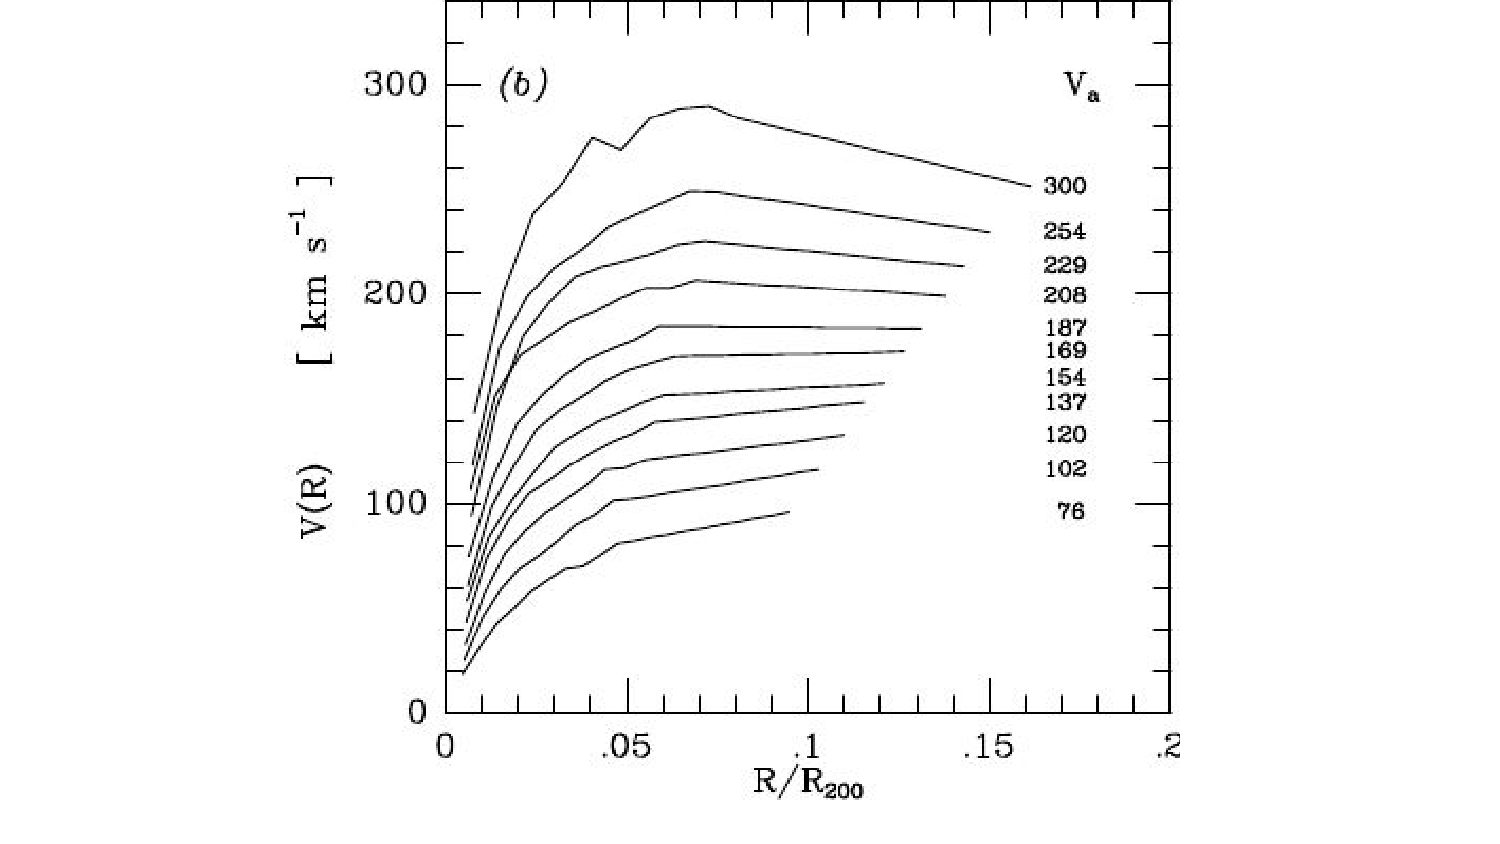
\includegraphics[width=\linewidth]{URC}
     \caption{\emph{Universal Rotation Curve spectrum, Used with permission from Ref.\citep{salucci}}}
     \label{fig:URC}
\end{figure}
  

  
    
 \begin{figure}[h!]
%\scalebox{0.25075}%
      \centering
      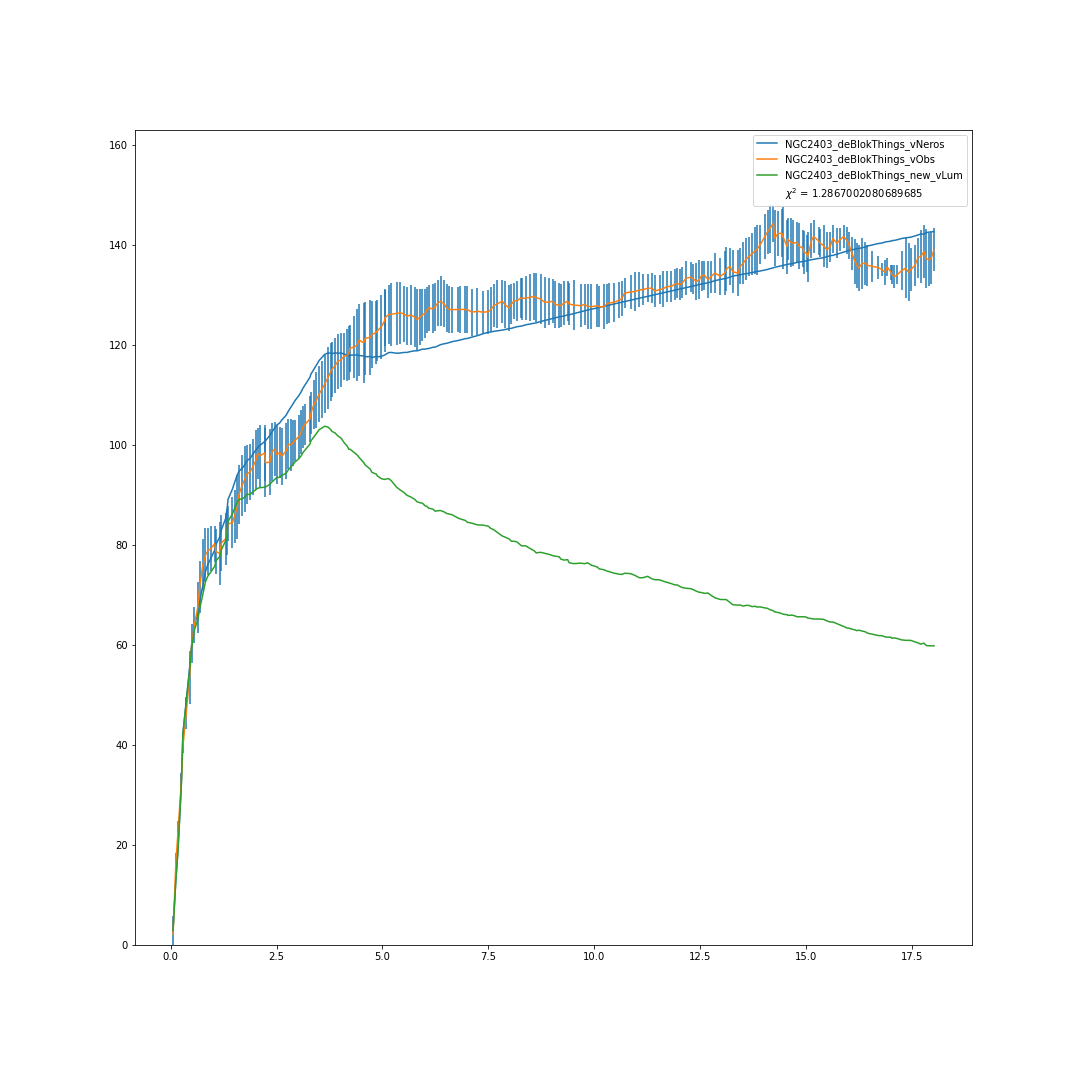
\includegraphics[width=\linewidth]{NGC2403_deBlokThings_XueSofue}
      \caption{\emph{Rotation Curve of NGC 2403 \cite{Blok1}.   Rotation curve data blue dots with  error bars,  Keplerian velocity from luminous mass estimated by   green line,   RCFM fit blue line.} }
      \label{fig:NGC2403}
  \end{figure}
%%%%%%
%%%%%%%%
%%%%%%
%%%%%%%
%%%%%%
%%%%%%
\section{Rotation Curve Fitting Formulae  \label{sec:dos}}
 \subsection{Dark matter rotation curve fitting formula}
 
  

 The standard dark matter rotation curve formula for rotationally supported galaxies, in the plane of the galactic disk,  is 

 \begin{equation}
v(r)^2_{obs}  =  v(r)^2_{lum}  +  v(r)^2_{dm}   
\label{eq:zonte1}
\end{equation} 

  where all velocities are assumed to be circular orbits about the rotation axis of the galaxy at  $r=0$. Terms in  $v_{obs}$ come  from observations of Doppler shifted spectra (Eq.~\ref{eq:modelLumA}), $v_{lum}$ from observations of total light  (photometry) interpreted by Population Synthesis Models as mass and hence orbital velocities (Eq.~\ref{zoochance1}),  and $v_{dm}$ represents  the missing   mass component by the following logic.
  
  
 Terms in  Eq.~\ref{eq:zonte1} are added in quadrature to reflect a   mass sum
  
\begin{equation}
    M(r)_{total}   = M(r)_{lum}   + M(r)_{dm}  ,  
\end{equation}

for a  Newtonian gravitational potential 

\begin{equation}
      \Phi(r)  = -G \int d^3r'  \frac{ \rho(r') }{r-r'} ,
      \label{eq:Newt}
      \end{equation}

which solves Poisson's equation

\begin{equation}
\nabla^2 \Phi(r)_{lum}  = 4\pi G \rho(r),   
    \label{whatsgood}
\end{equation}

for $G$ Newton's universal gravitation constant, and 
$\rho(r')$  the mass density. 
The gravitational  central force law   

\begin{equation}
 \frac{\partial \Phi(r)_{lum}}{\partial r}    =\frac{v(r)_{lum}^2}{r},   
    \label{zoochance1}
\end{equation}

  relates centripetal acceleration $v^2/r$ to the gradient of the potential.   In this way, the  quadratic velocity terms in   Eq.~\ref{eq:zonte1} represent enclosed masses as a function of radius in the disk, and the 
 difference $(M_{dyn}-M_{lum})$  is 
  the source   for the dark matter halo  
 $v(r)^2_{dm}$.  



\subsection{New Rotation Curve Fitting Model}



 
 To construct a new  rotation curve fitting formula (RCFM), we   replace dark matter  in  Eq.~\ref{eq:zonte1}, 
  with   a product of a free parameter $\alpha$,  a curvature ratio, and two  Lorentz-type transformations,   
   

\begin{equation}
v_{rc}^2 =  v_{lum}^2+\alpha \kappa^2 v_{1} v_{2} , 
\label{eq:zonteLCM}
\end{equation}  


We  directly modify  the standard dark matter rotation curve formula as a heuristic way to test this concept, and    
under the assumption that shifts in   spectra due to relative velocity and relative acceleration are separable, albeit perhaps not in exactly this way \cite{Jack,Cisn}.
 In what follows, all   terms  can be assumed to   functions of radius except the model's free parameter $\alpha$,  which is single valued for each galaxy fitted.

  
 The term $\kappa$ 
is a ratio of Newtonian gravitational potentials 

 \begin{equation}
\kappa=\frac{\Phi_{gal}}{\Phi_{mw}}, 
\label{eq:kappa2}  
\end{equation}  

 for $\Phi_{gal}$ representative of the reported estimates of the luminous mass in the galaxy being observed, and $\Phi_{mw}$ for the same in  the Milky Way.  Careful consideration of how to calculate and compare   gravitational potentials of   the galaxies relative to each other, since terms in $\Phi$ determine the metric term $g_{tt}$. Integration protocols are discussed in detail in Sec.~\ref{sec:gravDets}.
 

 
 In what follows, we will consider the data reported as the rotation curve velocity $v_{obs}$, Eq.~\ref{eq:zonte1}, at the level of the   observations of  Doppler shifted spectra $\omega'$, 

 \begin{equation}
 \frac{v_{obs}(r) }{c}=
\frac{  \left( \frac{\omega'(r)}{\omega_o}\right)^2 -  \left( \frac{\omega_o}{\omega'(r)} \right)^2 }{  \left( \frac{\omega'(r)}{\omega_o}\right)^2  +  \left( \frac{\omega_o}{\omega'(r)}\right)^2 }. 
\label{eq:modelLumA}
\end{equation} 

 This   relationship is from a Lorentz  boost in Minkowski spacetime,   applicable to 
  relative   motion of inertial frames, and can be rewritten in hyperbolic form\cite{rindler2013essential} as


     \begin{equation}
         \frac{v}{c} = \tanh \zeta = \frac{e^\zeta - e^{-\zeta}}{e^\zeta + e^{-\zeta}} .   
         \label{boost}
     \end{equation} 

On inspection, we will identify   the field-frame relationship with the   Lorentz exponential    $e^\zeta = \omega'(r) /\omega_o$, for
$\zeta$ the   rapidity  angle.  This is    the  frame-field relationship we want to modify for use between slightly curved galaxy frames. 
For  motivation of this    technique,  see discussion   in  Sec.~\ref{sec:gravDets}, which   is  based upon the conservation properties of the timelike Killing vector field,  evaluated  in   two distinct galaxy manifolds at the same $r$ (see Eq.~\ref{clocktime}).  


 Terms in $v_1$ and   $v_1$ will Lorentz map between galaxy frames one-to-one in radius, by identifying the Lorentz exponential term   between  galaxies  as
   
     \begin{equation}
     e^{\xi}=  \frac{\omega_{mw}}{\omega_{gal}}  =\sqrt{\frac{g_{tt}|_{gal}}{g_{tt}|_{mw}}}
      \label{eq:gravRS}
    \end{equation}
    
for  
 Schwarzschild   clock term $g_{tt}$
 
  \begin{equation}
      g_{tt}= -( 1 - 2\Phi/ c^2).
      \label{clocktime}
  \end{equation} 
  
 This is the    weak field Schwarzschild   time metric term in  Boyer-Lindquist coordinates \cite{Hartle}, and $c$ is the constant vacuum light speed.
  
  
 All spiral galaxy manifolds,  in the weak field Schwarzschild limit, can be     assumed to be covered with a timelike   Killing vector field 
   $\xi^t(r)$, where the norm of that field is related to the time metric coefficient  by  $\xi^b \xi_b =g_{tt}$ \cite{Wald}, for 
   
 
 
  
   
   \begin{equation}
       \frac{\omega_1}{\omega_2}  =\sqrt{\frac{g_{tt}|_{P2}}{g_{tt}|_{P1}}} =\sqrt{\frac{|\xi^t\xi_{t}|_{P2}}{|\xi^t\xi_{t}|_{P1}}}. 
      \label{eq:grav}
    \end{equation}
    
   Extension of this formalism to relate two separate manifolds will be explored in the next section, and based on Wolfgang Rindler's acute observation  that    ``the center of each galaxy provides a basic local standard of nonacceleration ... so then can be treated like a local inertial frame relative to its own center.''\cite{rindler2013essential}.




    
 Terms in $v_1$   are then 
 
   \begin{equation}
       v_1 = \sinh \xi. 
   \end{equation}
 
 

The second Lorentz-type map is $v_2$, which transforms between the  curved 2-frame in Eq.~\ref{eq:gravRS} and  the flat 2-frame where we make observations. That this second step is necessary is supported by the constancy of the speed of light.   
The   $v_2$   Lorentz exponential term  is identified as a convolution of the curved and flat frames
 
\begin{equation}
    e^{\eta}=   e^{(\xi+f)/2}.
\end{equation}

 (FIX INDICES ++++ MESSSY GREEK AND ROMAN)

The flat field-frames where we make observations  are identified with the frequency shifts $\omega'(r)_{lum}$ expected  estimates of   Keplerian rotations, $v_{lum}$,   

 
 \begin{equation}
 \frac{v_{lum}(r) }{c}=
\frac{  \left( \frac{\omega'(r)_{lum}}{\omega_o}\right)^2 -  \left( \frac{\omega_o}{\omega'(r)_{lum}} \right)^2 }{  \left( \frac{\omega'(r)_{lum}}{\omega_o}\right)^2  +  \left( \frac{\omega_o}{\omega'(r)_{lum}}\right)^2 }. 
\label{eq:lumlorentz}
\end{equation} 
 
 
  We assume Keplerian rotation curves are     the best estimate of flatness since dark matter is not required to  reproduce the rotation curve of our Solar System, so 
the flat two-frame Lorentz exponential term is 

\begin{equation}
    e^{f}=\frac{\omega_{l}}{\omega_o}= \sqrt{\frac{1+\beta}{1-\beta}},  
    \label{eq:flat}
\end{equation}  
     
and then, the best  $v_2$  transformation is 

\begin{equation}
v_{2} =  \cosh \eta.
\label{eq:hyperbolico}
\end{equation}


Note, when viewed as    Rindler's accelerated coordinates\cite{MTW,Wald, rindler2013essential}, $v_1$ is  timelike   and $v_2$ is spacelike.  This approach    assumes that the tetrad formalism allows us to place field-frames at each point in a galaxy manifold, parametrized with small deviations from flatness due to gravity in $g_{tt}$, and  then to Lorentz boost between these manifolds to predict rotation curve observations. 
  Fitting details and analysis are reported in Sec.~\ref{sec:analysis}. This concept has been previously explored in a series of papers \cite{Cisneros:2013vha,Cisneros:2014fea,Cisneros2015,Cisn2016}, though we here report an improved class of Lorentz-type transformations and a larger, more representative sample of galaxies. 
  
  
  
  
   
    
  
 
%%%%%%
%%%%%%%
%%%%%%
%%%%%%%  
%%%%%%
%%%%%%%  
\subsection{Integration protocols \label{sec:gravDets}}

 In what follows, we    assume  luminosity   is a Lorentz scalar, therefore invariant under the assumption of a good distance estimate. This   means   we take reported   estimates of total light as faithful tracers of mass. 
   In addition, we assume   
   Doppler shifted spectra is part of a Lorentz 4-vector, and so    must transform in a Lorentzian sense. 
   We   also assume   the additional Tetrad-formalism assumption of a local Lorentz symmetry attached at each point in the manifold.  This will allow comparison of gravitational manifolds in $g_{tt}(r)$, given a careful calculation  of the gravitational potentials. 
   
   
 
Based on   Rindler's statement, relating two such Killing fields,  one-to-one in radius, will be accomplished  by synchronizing the galaxy centers. 

 




 
   
  To compare galaxy centers, and  
 synchronize   clock fields   in $g_{tt}$, we   require aligning terms in  the Newtonian  gravitational potentials  $\Phi $. 
 Classically, $\Phi$ is integrated from the large $r$ limit   $r->\infty$,  to the inside small $r\approx 0$ limit. 
This integration order is an implicit assumption of a flat embedding spacetime, where for   energy conservation all potentials go to zero at the large $r$ limit. 
However,  as observations have shown \cite{Pomarede:2020pme,Hoffman:2017ako}, 
the external environments of galaxies are   extremely   diverse,   depending on where and when  in the large-scale structure streamlines and Hubble flow the galaxy evolves. Some galaxies evolve in relative isolation, whereas others evolve in   huge clusters of galaxies. In addition, a priori,  we have no idea of the curvature of the universal embedding spacetime,  the background vacuum energy content of the universe (CITE), or the  global   value of the Hubble constant(CITE).  What we do know  is that all galaxy clocks read the same time at the event horizon. And further, since
  what we measure    is differences in potentials, our ignorance is of no account if we synchronize galaxy centers. At the event horizon, which for our investigations is essentially $r=0$,  all 
  galaxies have  the same notion of zero. In practice,  this   amounts to reversing the 
    order of integration of $\Phi$, so that  we 
integrate  from the small $r$ limit out  to the large $r$  extent of the data  

 \begin{equation}
     \Phi  =   \int^{R-big}_{r-small} \vec{F_r}\cdot\vec{dr}  . 
      \label{eq:Newt2}
      \end{equation}
 
   We   assume that Newtonian potentials integrated in this way parametrize Killing fields,     from the same standard of rest at the galaxy center, so   Lorentz-type transformations can be used to compare galaxy frames foliated in $g_{tt}(r)$. 
   
     Potentials calculated in this way still obey the central force law for test particles moving in circular orbits in Eq.~\ref{zoochance1} and Poisson's equation Eq.~\ref{whatsgood}.

Since these potentials, and $g_{tt}$, will characterize the frames, we note that the tetrad formulation of General Relativity adds a local Lorentz symmetry


\begin{equation}
    g^{\mu \nu} = \eta^{\alpha \beta} e^\mu_a  e^\nu_b
\end{equation} 

for $e^\mu_a$ here representative of an orthonormal basis vector. The basis vectors now carry the information regarding the physical spacetime, but the tetrad at each point is Lorentzian and so can endure 3 boosts and 3 rotations \cite{BertschingerClassTetrads}. 


   All terms in $\Phi(r)$ used in this paper  are    integrated from estimates of the baryonic mass, as reported in the      SPARC  library \cite{2016Lelli}.  
   Assumptions in their reported luminous mass models  are included in Sec.~\ref{sec:analysis}. 
%%%%%%
%%%%%%%
%%%%%%
%%%%%%%
\subsection{Geometry and Mass-to-light ratios}

Studies of the mass-to-light ratios in galaxies began with Schwarzschild's early investigations \cite{1954AJ.....59..273S} and have evolved into a set of best practices, but modeling of the 
dark matter halo remains severely   underconstrained with correlated parameters including radius, slope, scale length, and halo core radius.     
The technique presented here, whether fundamental or no,  has the advantage of replacing the dark matter term  with a product of terms based only on estimates of the luminous mass and   one free parameter.


It is commonly assumed that   the stellar bulge, gas halo and   dark matter halo are spherically symmetric, but that the stellar disk is axially symmetric. We use 
the Schwarzschild metric   for clarity of the construction;  a static, stationary, spherically symmetric solution of Einstein's equations.
Flattened disks produce gravitational potentials which are weaker than a sphere of the same mass\cite{Chatterjee}. However, numerical integration of the disk is a computationally intensive and requires assumptions of  boundary conditions,   relevant physical scales,  etc. which add extra free-parameters\cite{2011A&A...531A..36H}. We 
  introduce the error of spherical symmetry   for the disk to maintain a clear presentation in the plane of the galactic disk, acknowledging  that inside of $r< R/3$, we   overestimate the gravitational potential, and  mass-to-light ratio by approximately $15\%$ (see Fig.~\ref{fig:my_geom}),  where R is the radius of the stellar disk configuration.  (CHECK WITH STACY). 


This introduced error does not change  the line shape, and   does not introduce any artifacts outside of $R/3$, where rotation curves become flat,  as the potentials for disk and sphere are commensurate there. The assumption of spherical symmetry is commonly used   in evaluation of the   rotation curve velocities from integrated potentials \cite{2022A&A...664A..40M,PhysRevD.70.083509}. 
 
\begin{figure}
    \centering
     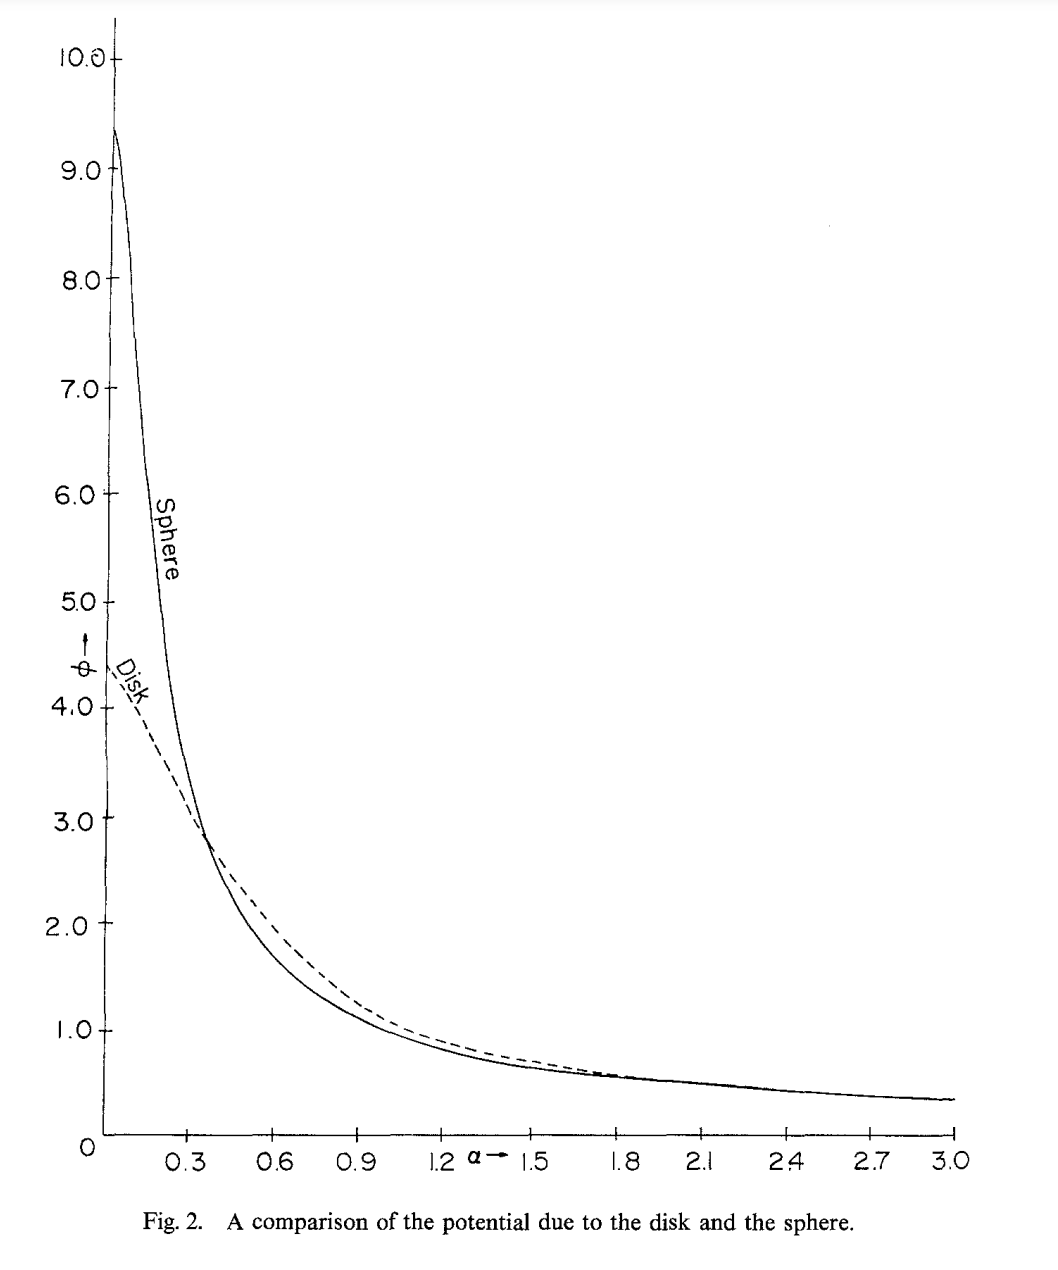
\includegraphics[width=\linewidth]{Chatterjee_SphereDisk.png}
    \caption{A $\alpha = r/R$ for $R$ the radial extent of the stars \cite{Chatterjee}}
    \label{fig:my_geom}
\end{figure}

  
  
%%%%%%
%%%%%%
%%%%%%% 
%%%%%%
%%%%%%
%%%%%%%  
%%%%%%
%%%%%%%  
%%%%%%
%%%%%%%
\section{Data \label{sec:data}}
%  

We will parametrize gravitational frames from estimates of luminous mass reported kinematically as  $v_{lum}$, Eq.~\ref{eq:zonte1}. These velocities  are constructed from photometric observations of surface brightnesses, interpreted   by a Population Synthesis Model (PSM)\cite{10.1093/mnras/sty3223} as     masses. 
PSM rely upon a complex  suite of  assumptions regarding galaxy evolution, metallicities and initial mass functions  \cite{BelldYong,10.1093/mnras/sty3223}. PSM predict   mass-to-light ratios  $\gamma_i$
 which translate  luminosity into mass
 
  \begin{equation}
v(r)_{lum}^2 = \gamma_b v(r)_{bulge}^2 +  \gamma_d v(r)_{disk}^2 + v(r)_{gas}^2.   
\label{eq:zonte3}
\end{equation} 
 
 
 
  Gas fractions are  not scaled because the observation techniques do not require a PSM to yield masses.  Baryonic mass contributions (disk, bulge and gas) are summed quadratically to represent a mass sum in the same way as in   Eq.~\ref{eq:zonte1}.

\subsection{SPARC dataset}
 
 We fit a sample  of  175 nearby galaxies with extended rotation curves from atomic hydrogen (HI) collected from the literature and reported and standardized in  the SPARC data base library (Spitzer Photometry and Accurate Rotation Curves\cite{2016Lelli}). HI provides the most reliable
 rotation curves because it dynamically cold, traces circular orbits, and can be observed several effective radii past the stellar disk. 
 This sample of rotationally supported galaxies also spans the widest range of masses and morphologies currently available. In addition, these galaxies are  accompanied by mass models which come from surface photometry in the 
   near infrared  at 3.5$\mu m$, which is widely believed to be the best tracer of stellar mass and in population synthesis models  gives mass-to-light (M/L) ratios which are almost constant independent of star formation history,  versus those from   optical measurements\cite{BelldYong,10.1093/mnras/sty3223}.  Stellar M/L ratios   translate between photometry and dynamics. 
   
   Mass models include Luminous mass contributions from a stellar bulge, stellar disk, gas fraction, as shown in Eq.~\ref{eq:zonte3}. Gas fractions are calculated from surface density profiles of HI by the formula from (CITE Casertano (1983)) which solves the Poisson equation for a disk geometry and
   includes the total mass of the HI scaled by a factor of 1.33 to include helium abundances . Stellar bulges are assumed to be spherical, and stellar disks are assumed to go to exponentially approach zero at  infinity unless there is a clear delineation of the end of the galaxy disk. It is interesting to note that \citet{2016Lelli} state that errors come from uncertainties in the M/L ratios rather than the geometry assumptions
   
 
%The gas contribution is calculated using the formula from Casertano (1983), which solves the Poisson equation for a disk
%with finite thickness and arbitrary density distribution. We
%assume a thin disk with a total mass of 1.33 M H I, where the
%factor 1.33 considers the contribution of helium. Vgas is either
%omputed using H I surface density profiles or taken from
%published mass models. For D512-2, D564-8, and D631-7,
%H I surface density profiles are not available; hence, we
%compute Vgas assuming an exponential profile with a scale
%ength of 2Rd. This is a reasonable approximation for such latetype galaxies (e.g., Swaters et al. 2002). We neglect the
%contribution of molecular gas because CO data are not
%available for most SPARC galaxies. 
   
 %Their final science sample is made of 153 galaxies.
 
 %Disk-Halo degeneracy: McGaugh says that van Albada talks about it here \cite{1985ApJAlbada}, but really just means the conspiracy between the peak rotation curve velocity and the luminous mass - and that it's hard/impossible to tell if the inner velocity is due to the stars or the halo. This is why Stacy uses the near infrared $3.6 \mu m$ wavelength that is the best tracer for stellar mass. Stellar Population Synthesis models suggest that in this wavelength band the M/L is essentially constant across a wide range of galaxy morphologies and  masses, independent of star formation history .
 

 
 van Albada: Assume a galaxy is composed of a stellar bulge and a disk, and assume that each has a constant M/L ratio. At 1/3 the effective radius (half light radius) the maxima of the rotation curve happens for spheroid and disk. 
   with  the RCFM in order to compare results with    MOND and RAR and dark matter fits to the same data set   \cite{McGaugh_2014,Li_2018}. 


%%%%%%
%%%%%%
%%%%%%%
\subsection{Milky Way}
 
All terms in the RCFM presented here require a static assumption of the Milky Way  baryon profile. 
Determination of the gravitational potential of the luminous mass in the Milky Way (MW) galaxy is a famously under-constrained problem of   taking observations of the system, from within the system. Many clever approaches have been used to constrain the    problem \cite{1991ARA&A..29..409F}.
However, outside of our position at 8 kpc in the disk of the MW, the observations have been notoriously difficult to interpret. In  recent large surveys of millions of  stars in the Milky Way  we begin to see  constraints to these models from  SDSS APOGEE-2 \cite{2022ApJS..259...35A},  \cite{10.1093/mnras/stt814}.  

However, in the absence of a definitive conclusion to the story of the mass of the MW, we choose three different static MW baryon distributions from \cite{Xue}, \cite{Sofue}, and CITE(MCGAUGH-figure out where he p ublished the MW stuff). 
Other static MW profiles are available at the Github repo: Cisneros-Galaxy/RCFM. 

\cite{2008ApJ...673..864J} Mario Juric's paper - has info  on the MW from SDSS, surveyed like 48,000 stars. Gotta get him to look at our MW models. 

{\color{red}  }
{\color{red} \rule{\linewidth}{0.5mm}}

 

IN \cite{Li2016ModellingMD} the bulge is more like Sofue. Not flat like McGaugh. 
To understand why. 
``using the recently released Gaia billion-star map8
, we propose a
Galactic disk mass distribution model which is based on the star density distribution
rather than the brightness and mass-to-light ratio. ''
TROUBLE: ``we obtain a flat rotation curve
which reproduces the key observed features with no need for a dark halo''.

 
  
 
%%%%%%
%%%%%%
%%%%%%%
\section{Analysis and Constraining the free parameter \label{sec:analysis}}

%%TO DO: PUT ASSUMPTIONS FOR SPARC LUM MODELS - " Assumptions in their reported luminous mass models  are included in Sec.~\ref{sec:analysis}. "

In RCFM fits reported here, the    bulge and disk mass-to-light ratios are allowed to vary freely (See Eq.~\ref{eq:zonte3}), though the average values are within stated criteria   \cite{2016Lelli} of $\pm 20\%$. The gas fractions (HI scaled for Helium abundance) are fixed though addition of molecular gas could increase mass fractions in the inner kiloparsec of a galaxy(CITE RENE WB), and it is common (CHECK-Y-YO) to scale the observed 21-cm flux by $4/3$ to account for molecular gas \cite{2004ApJ...609..652M}.


\subsection{NGC 3198 and other galaxies}
\cite{1985ApJAlbada} studies this galaxy, which MOND has troubles with. This galaxy has an exponential disk, they use 2 components -  a thin exponential disk de Vaucouleurs 1959;
Freeman 1970, and dark matter spheroid Young (1976). Dijo algo about using an infinite disk - uggg. 
 
\cite{Toky} mentions that MOND fails to fit NGC 3109, which we fit exceedingly well ($\chi^2 = 0.32$).
%%%%%%
%%%%%%%%
%%%%%%
%%%%%%%
%%%%%%
%%%%%%
\subsection{Correlation to  the model's free parameter }


 In \cite{2016Lelli}, it says that they have fifty  galaxies with highly accurate distance: (45) from tip of the red giant branch, (3) from Cepheids, (2) from supernova, with errors in distance on the order of $5\% - 10\%$. We use this subset to investigate   the free parameters for these galaxies with respect to a guess at its physical significance. 
 
 
 %NEED TO SEE IF WANT TO INCLUDE SN GALS TOO... train the model's free parameter we select a subset of galaxies who have Cepheid or Tip of the Red Giant Branch distance measurements. 
 % DO WE WANT TO DO THIS, OR JUST DO THAT SUBSEQUENT?> When the free parameter is fixed to a constant value, we will then run on the entire SPARC data set,
We also exclude galaxies  which have an inclination greater than $85^o$ as impossible to constrain a proper surface brightness profile, and those at inclinations less than $35^o$ as being impossible to accurately report line of sight Doppler shifts.   
  By this criteria, we select 46 galaxies (See Table \ref{tab:Tset}. 
  
  
  \begin{table*}[]
      \centering
      \begin{tabular}{|c|c|c|c|c|c|}
      \hline \hline
Galaxy Name & Hubble Type(1)& 	Distance (Mpc)&Mean Error on D (Mpc)& 	Distance Method (2)& 	Inc (deg)\\
    \hline \hline\\
CamB&   	10&    3.36&  	0.26&   2&  65\\
D564-8& 	10& 	8.79& 	0.28& 	2& 	63\\
D631-7& 	10& 	7.72& 	0.18& 	2& 	59\\
DDO154& 	10& 	4.04& 	0.2& 	2& 	64\\
DDO168& 	10& 	4.25& 	0.21& 	2& 	63\\
ESO444-G084& 10& 	4.83& 	0.48& 	2& 	32\\
IC2574& 	9& 	3.91& 	0.2&    	2& 	75\\
NGC0024& 	5& 	7.3& 	0.36&   	2& 	64\\
NGC0055& 	9& 	2.11& 	0.11&   	2& 	77\\
NGC0247& 	7& 	3.7& 	0.19&   	2& 	74\\
NGC0300& 	7& 	2.08& 	0.1&    	2& 	42\\
NGC0891& 	3& 	9.91& 	0.5&    	2& 	90\\
NGC1705& 	11& 	5.73& 	0.29& 	2& 	80\\
NGC2366& 	10& 	3.27& 	0.16& 	2& 	68\\
NGC2403& 	6& 	3.16& 	0.16&   	2& 	63\\
NGC2683& 	3& 	9.81& 	0.49&   	2& 	80\\
NGC2841& 	3& 	14.1& 	1.4&    	3& 	76\\
NGC2915& 	11& 	4.06& 	0.2& 	2& 	56\\
NGC2976**& 	5& 	3.58& 	0.18&   	2& 	61\\
NGC3109& 	9& 	1.33& 	0.07&   	2& 	70\\
NGC3198& 	5& 	13.8& 	1.4&    	3& 	73\\
NGC3741& 	10& 	3.21& 	0.17& 	2& 	70\\
NGC4068& 	10& 	4.37& 	0.22& 	2& 	44\\
NGC4214& 	10& 	2.87& 	0.14& 	2& 	15\\
NGC5055& 	4& 	9.9& 	0.3&    	2& 	55\\
NGC5907& 	5& 	17.3& 	0.9&    	2& 	88\\
NGC6503& 	6& 	6.26& 	0.31&   	2& 	74\\
NGC6789& 	11& 	3.52& 	0.18& 	2& 	43\\
NGC6946& 	6& 	5.52& 	1.66&   	2& 	38\\
NGC7331& 	3& 	14.7& 	1.5&    	3& 	75\\
NGC7793& 	7& 	3.61& 	0.18&   	2& 	47\\
NGC7814& 	2&  	14.4& 	0.66& 	2& 	90\\
PGC51017**& 	11& 	13.6& 	1.4& 	2& 	66\\
UGC01281& 	8&   	5.27& 	0.24& 	2& 	90\\
UGC04305**& 	10& 	3.45& 	0.17& 	2& 	40\\
UGC04483& 	10& 	3.34& 	0.31& 	2& 	58\\
UGC07151& 	6& 	6.87& 	0.34&   	2& 	90\\
UGC07232& 	10& 	2.83& 	0.17& 	2& 	59\\
UGC07524& 	9& 	4.74& 	0.24& 	    2& 	46\\
UGC07559& 	10& 	4.97& 	0.25& 	2& 	61\\
UGC07577& 	10& 	2.59& 	0.13& 	2& 	63\\
UGC07866& 	10& 	4.57& 	0.23& 	2& 	44\\
UGC08286& 	6& 	6.5& 	0.21&   	2& 	90\\
UGC08490& 	9& 	4.65& 	0.53&   	2& 	50\\
UGC08837& 	10& 	7.21& 	0.36& 	2& 	80\\
UGCA281& 	11& 	5.68& 	0.28& 	2& 	67\\
UGCA442& 	9& 	4.35& 	0.22& 	    2& 	64\\
UGCA444& 	10& 	0.98& 	0.05& 	2& 	78\\
    \hline \hline           
      \end{tabular}
      \caption{Table from  \citet{2016Lelli}. 
      (1) Hubble type:  from (CITE) de
Vaucouleurs et al. (1991), (CITE) Schombert et al. (1992), or (CITE) NED3
of: 0 = S0, 1 = Sa, 2 = Sab,
3 = Sb, 4 = Sbc, 5 = Sc, 6 = Scd, 7 = Sd, 8 = Sdm,
9 = Sm, 10 = Im, 11 = BCD.  (2) Distance method: : 1 = Hubble flow,
2 = tip of the red giant branch, 3 = Cepheids, 4 = Ursa Major
cluster of galaxies, 5 = supernovae. ** notes galaxies excluded from fit bc fail to fit, and see if we want to include SN gals, there's only 3...and 2 of the 3 that fail are weirdi rotations (non-circular)}
0      \label{tab:Tset}
  \end{table*}
  
  %%NOTE: Homies for SPARC used hybrid rotation curves on 56 galaxies, combining H-alpha  (inner) with HI (outer) Check if our "bad" gals are part of thi, or if is algo mas. Despite the high spatial resolution, Hα rotation curves are sometimes quite uncertain due to the patchy distribution and complex kinematics of Hα gas, especially for low-mass and LSB galaxies. We %use only H I data for the several objects:DDO 154, IC 2574, NGC 3109, NGC 5033, NGC 5055,NGC 6946, NGC 7331, and UGC 2259.(THESE ARE ALL GOOD
  %H I and Hα rotation
%curves, however, agree within the errors

%or face-on ones.We assign a quality flag (Q) to each rotation curve using the following scheme: Q = 1 for galaxies with high-quality H I data or hybrid Hα/H I rotation curves (99 objects); Q = 2 for
%galaxies with minor asymmetries and/or H I data of lower
%quality (64 objects); Q = 3 for galaxies with major asymmetries, strong noncircular motions, and/or offsets between H I
%nd stellar distributions (12 objects). Galaxies with Q = 3 are%
%not suited for detailed dynamical studies: we build mass models
%for completeness but do not consider them in our analysis.
%K BIEN_ Both UGC04305_rotmod and PGC51017_rotmod have Q=3. discard anyhow. but not: NGC2976_rotmod, it's a Q=2. Plus we have a few other galaxies in this subset with a Q=3,,,


  We search the free parameter $\alpha$ space of this subset of SPARC galaxies by plotting the single valued free parameter of each galaxy   versus a proxy for the gradient in the gravitational potential
  
   \begin{equation}
     \rho = L_{total}/R_{eff}.
 \end{equation}
 
 The  estimates of the  total luminosities $L_{total}$ at $3.6 \mu m$,  assume a solar
absolute magnitude of 3.24 at $3.6 \mu m$ (CITE Oh et al. 2008). The effective radius $R_{eff}$ is    the radius encompassing half of the total luminosity \citet{2016Lelli}.  
 

 We find $\alpha$  to be   strongly correlated to  this quantity. 
  
 \begin{figure*}[h]
\scalebox{0.5}%
{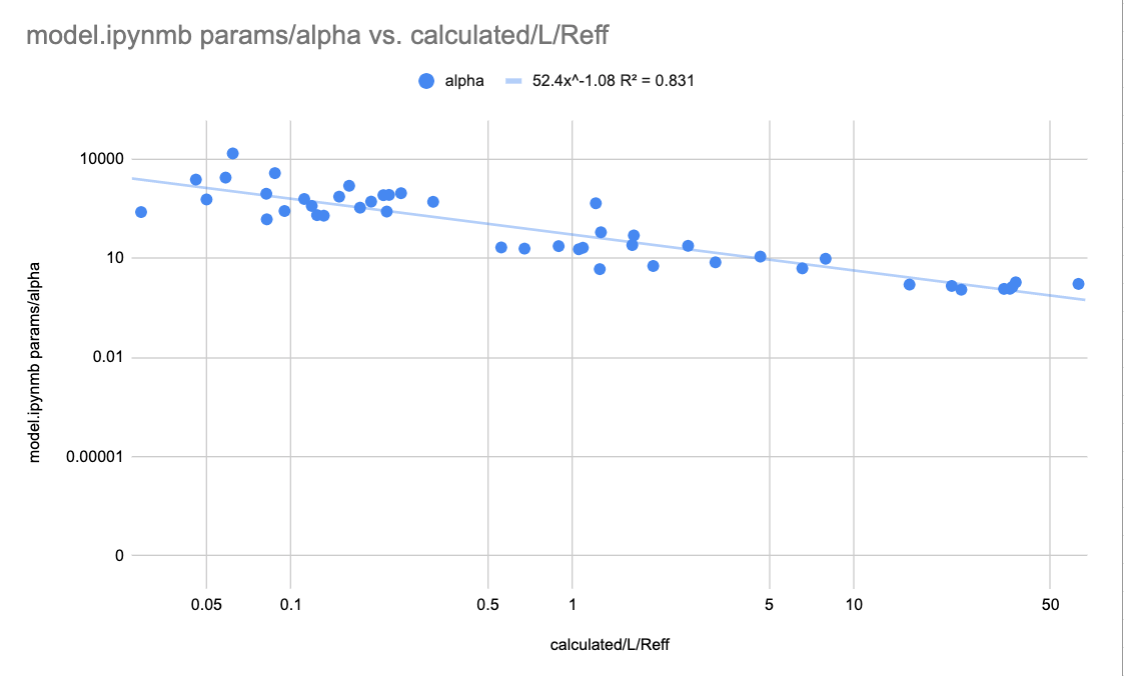
\includegraphics{alpha_10_18_22.png} }
\caption{ Remake this graph, nice   }
\label{alpha2}
\end{figure*}  
 
for 
\begin{equation}
    \alpha = 
\end{equation}



We might assume that $\alpha$ is a ratio of the same quantity for  the Milky Way $\rho_{mw}$ with respect to the other   galaxy $\rho_{gal}$  

\begin{equation}
\alpha=\left(\frac{\rho_{mw}}{\rho_{gal}}\right)^{b}  ,
\label{correl}
\end{equation}

then we arrive at a similar fit (See Fig.~\ref{alpha1}.

 
\subsection{MOND  \& RAR Comparison}



 
 In MOND,  classical gravity is transitioned to  a paradigm where the luminous mass is the only mass  but    the acceleration scale of gravity changes on the enormous distance scales of galaxies. MOND amounts to a phenomenological law of galaxy rotation curves, though does struggle in some galaxies.  Relativistic extensions of MOND have been summarized by  \citet{Famaey2012} and include notably the work of CITE(BEKENSTEIN), though all approaches require modifications to Einstein's well tested gravitational theory (CITE). 
  BY transitioning the MONDian concept of changing acceleration scales to changing  relative curvatures, we implicitly replace MOND's acceleration scale with the baryonic potential of the Milky Way, and find a more 
  efficient and flexible model than MOND. We are successful at fitting galaxies at Cepheid distances (GIVE NAME) that MOND struggles with, and we propose that this increased power is due to the more flexible use of the changing acceleration scale when pinned to the Milky Way and allowed to be the other frame in all transformations. 
  
While reported error    estimates on rotation curve velocities  have not been standardized across the field~\citep{Blok,Gent},     one can reliably   compare fits to the same data with the same  errors. The     reduced $\chi^2_r$ values printed on each graph and in table (MAKE TABLE), demonstrate the higher efficacy of the RCFM. 
 
  \citet{McGaugh2016RAR} is the paper where they present new fitting formula (compare to MOND), but en verdad, no me importa a mi. 
  
 
 
 
 
% \cite{McGaugh2016RAR} is the other one. This one describes the sample. 175 SPARC galaxies. Describes all the assumptions for the disk, gas, bulge models, the band used and reasoning, rotation curve data from HI, 
 
% They only fit a subset (153 of 175) of these galaxies.I get 128, I guess I'm cutting endpoints of 85 and 30 and they include. Plus I exclude like five that I think fail to fit
 
 
 \section{  Conclusions \label{sec:conclu}  }
 

{\color{red} This heuristic replacement of dark matter is not a fundamental derivation, but    one supposes if it is possible to quantify these
excesses in shifted spectra using only luminous mass as we do in this paper,  then a       derivation from first principles should   exist.  The curious conspiracy of the luminous mass to   determine the dark matter  is here more compactly explained and characterized as the imprint of our Milky Way on Doppler shifted spectra we receive from external galaxies. Not only is this a more efficient way to predict rotations curves as judged by the average reduced $\chi^2$, but it is also a  more conservative choice than either MOND or dark matter which both require new physics \cite{de_Blok_2010}.  
  
 
 

  
 
%Places where dark matter is invoked. Structure formation: put spherical model replace flat, solve. Galaxy clusters, same,put flow lines on surfaces supported by dark energy. Tully Fisher: temp dependence with mass - but read Beckenstein's description carefully. Hemakes some points.  
   
 
We   present here a new picture of flat-rotation curves which does not   modify Einstein gravitational physics, but adds a new technique to the standard transformations of   relativity. }
  
 

%%%%%%
%%%%%
%%%
%%
%
%%%%%%


 % \caption{Results   for SPARC Luminous mass profiles  [NOT UPDATED]\label{sumRESULTS}}
 % \begin{tabular}{@{}llccccccc@{}}
 % \hline
 %  Galaxy     	  &Ref.~&  \multicolumn{3}{c}{\underline{ Other Model Fit Results}}	& & \multicolumn{3}{c}{\underline{LCM Fit Results }}  \\
%\hline
%   	 	& & &  $M/L_{disk}$		& $\chi^2_r$	&&$M/L$&$r_e$&$\chi^2_r$ \\ 
% \hline
%F 563-1	& 2	%& 			
%					&NFW	&--	 		&-- & 	&1.13 	&2.84 	&0.06 \\
%M 31* 	& 12 	%&7.5
%					&ISO	 	 &7.50		&0.36 & 	&5.88	 &4.80 	&0.04  \\
%M 33		& 5	 %&	K 		
%					& NFW 	&0.70		&2.46&  	 &1.98	 &1.46	& 0.17 \\
%NGC 891*	& 11 	% &3.6$\,\umu$m 
		%			&MaxLight &0.9 			&1.10  & 	 &--  	 &	&0.25 \\ 
%NGC 925 	&3	%&3.6$\,\umu$m
 			%		&ISO 	&0.18		 &2.40& 	&0.92	 &4.35	&0.11 \\
%NGC 2403	 & 3	%& 3.6$\,\umu$m
		%			& NFW	&0.41 	 	&4.56& 	&1.12	 	&2.18		& 0.88 \\
%NGC 2841*  &6-3	% & 3.6$\,\umu$m
%					&  James	&0.74 	 	&0.45 & 	&6.25	  &4.84	&0.11 \\
%NGC 2903  &10	 %&B	   		
%					&MOND   	&3.60 	 	&10.71& 	 &2.2	 	&2.81		&0.47\\
% NGC 3198 & 3 	%&3.6$\,\umu$m
%					 &NFW	&0.80	   	&5.40  &   	 &1.80 	 &5.10	&0.64   \\
%NGC 3521  & 8-6	 %&3.6$\,\umu$m 
%					&MOND	&0.71 	 	&0.97 & 	 &2.13  &3.23	&0.22 \\
%NGC 3726	& 10	%&B 			
%					&MOND	&1.00	 	&3.57& 	&1.06	 &2.70	&0.05 \\
%NGC 3953	& 10	%&B 			
%					&MOND	&2.7		 	&1.35& 	&1.79 	&2.60 	&0.35 \\
%NGC 3992	& 10	%&B 			
%					&MOND	&4.93	 	&0.50& 	&2.45 	 &4.77	&0.04 \\
%NGC 4088	& 10	%&B 			
%					&MOND	&1.16		 	&1.70& 	&5.58	 &2.70	&0.27 \\
%NGC 4138	& 10	%&B 			
%					&MOND	&3.5		 	&2.12& 	&3.67	 &1.46	&0.01 \\
%NGC 5055*	 & 3	%&3.6$\,\umu$m 
%					&  NFW	&0.79	 	&17.23&  	&5.87	 &3.29	&0.69 \\
%NGC 5533*	 & 10 %&B 			
%					&MOND	&0.6		  	&1.57 & 	&7.11 	  &3.23	&0.22  \\
%NGC 5907*	& 10	%&B 			
				%	&MOND	&1.6 		 	 &0.44& 	&2.04	 &3.45	%&0.09 \\
%NGC 6946*	&  10	 %& B			
%					&  MOND	& 0.5		 	&   3.03& 	&1.44 	 &0.76	&0.07  \\ 
%NGC 6946*	&  3	 %& B			
%					&  NFW	& 0.5		 	&   3.03& 	&1.44 	 &0.76	&0.07  \\ 
%NGC 7331	&8	% & 3.6$\,\umu$m
%					&James	&0.4 		 	& 0.45& 	&1.34	 &2.44	&0.09 \\
%NGC 7793  &14	%&B			
%					&ISO		&2.6		 	&1.08& 	&2.7	 &1.51	&0.11 \\
%NGC 7814* &11 	% & 3.6$\,\umu$m
%					&ISO   	& 0.68  	 	& 0.25& 	 &-- 	   &	&0.20 \\ 
%UGC 128		&6	%&				
	%				&James	&			&	&	&1.58	  &10.3	%&0.20\\
%UGC 6973	& 10	%&B 			
%					&MOND	&2.7		 	&23.5 & 	&--  	& 	&0.06 \\
%UGC 7524	& 6	%&B 			
%					&James	&--		 	&-- & 	&2.10 	&3.32 	&0.06 \\
% 1.~\citet{Bege}, 2.~\citet{JNav}, 3.~\citet{Blok} , 4.~\citet{Maria}, 
%5.~\citet{Cor03}, 6.~\citet{James},   7.~\citet{Batt},   8.~\citet{Gent},   9.~\citet{Bot},   10.~\citet{SanMcGa},
 % 11.~\citet{Frat},   12.~\citet{Car},   13.~\citet{giraud2000universal},   14.~\citet{Dicaire}, %15.~\cite{Klypin}. \\
%    \end{minipage}
%\end{table*} 


   

  \section[]{Acknowledgments}
 This work is dedicated to Emmett Till. This paper was written with gratitude on the usual, and accustomed  territories
of the Coast Salish, Cheyenne, Arapaho and Ute Tribal Peoples.
  The authors would like to thank  V.\,P.\,  Nair,   R.\, Walterbos, S.\ McGaugh, A.\, Klypin, K. Bender, C. Beetle and     T.\, Boyer.   \\
  
 
%The   dark matter problem  is currently woven into most faces of our cosmology (weaklensing, galaxy rotation curves, early structure formation, galaxy and cluster interactions).   We posit that not all of these problems are actually the same physics problem.  We will address in this paper only the dark matter problem in spiral galaxies, the so-called flat-rotation curve problem discovered by \citet{1978Rubin,Bosma78}. We believe the ideas presented here are extensible to the problem of galaxy and cluster interactions, and perhaps weak lensing, but not to early structure formation, which we believe to be a different physics problem. 


 \begin{figure}[h]
\begin{subfigure}{.5\textwidth}
  \centering
  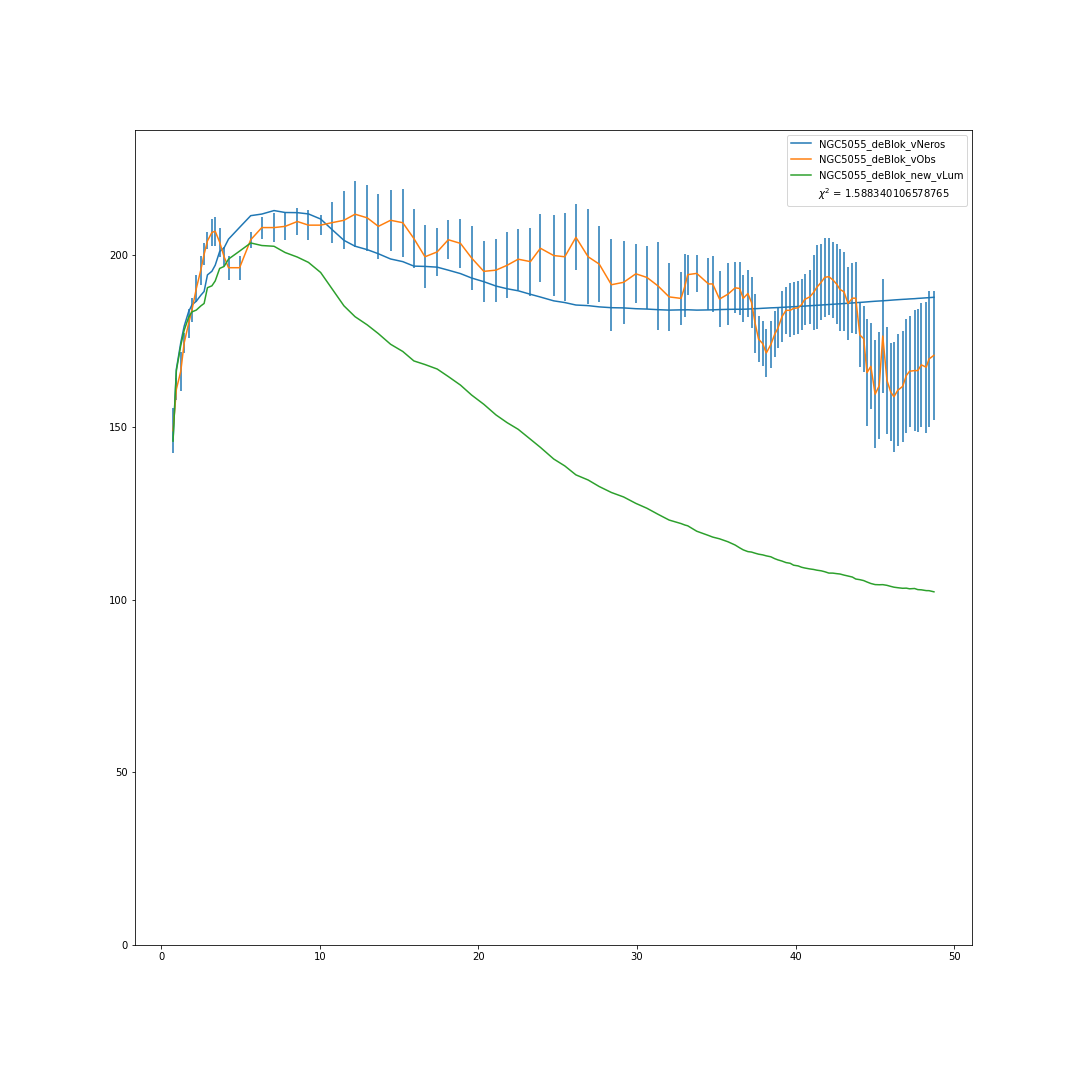
\includegraphics[width=.8\linewidth]{NGC5055_deBlok_XueSofue}
  \caption{deBlok\cite{Blok1}}
  \label{fig:sfig1}
\end{subfigure}%
\begin{subfigure}{.5\textwidth}
  \centering
  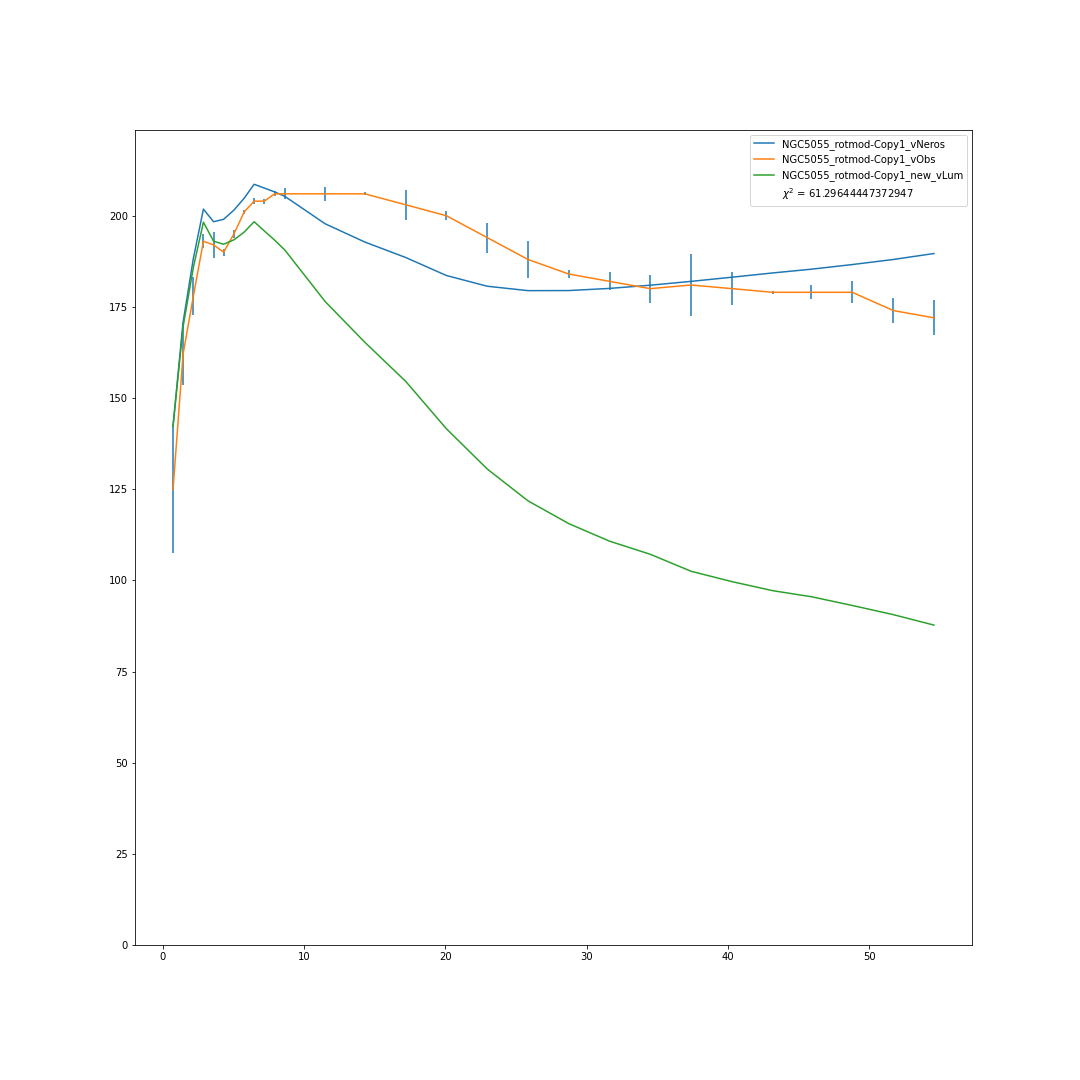
\includegraphics[width=.8\linewidth]{NGC5055_rotmod-Copy1_XueSofue}
  \caption{SPARC\cite{2016Lelli}}
  \label{fig:sfig2}
\end{subfigure}
\begin{subfigure}{.5\textwidth}
  \centering
  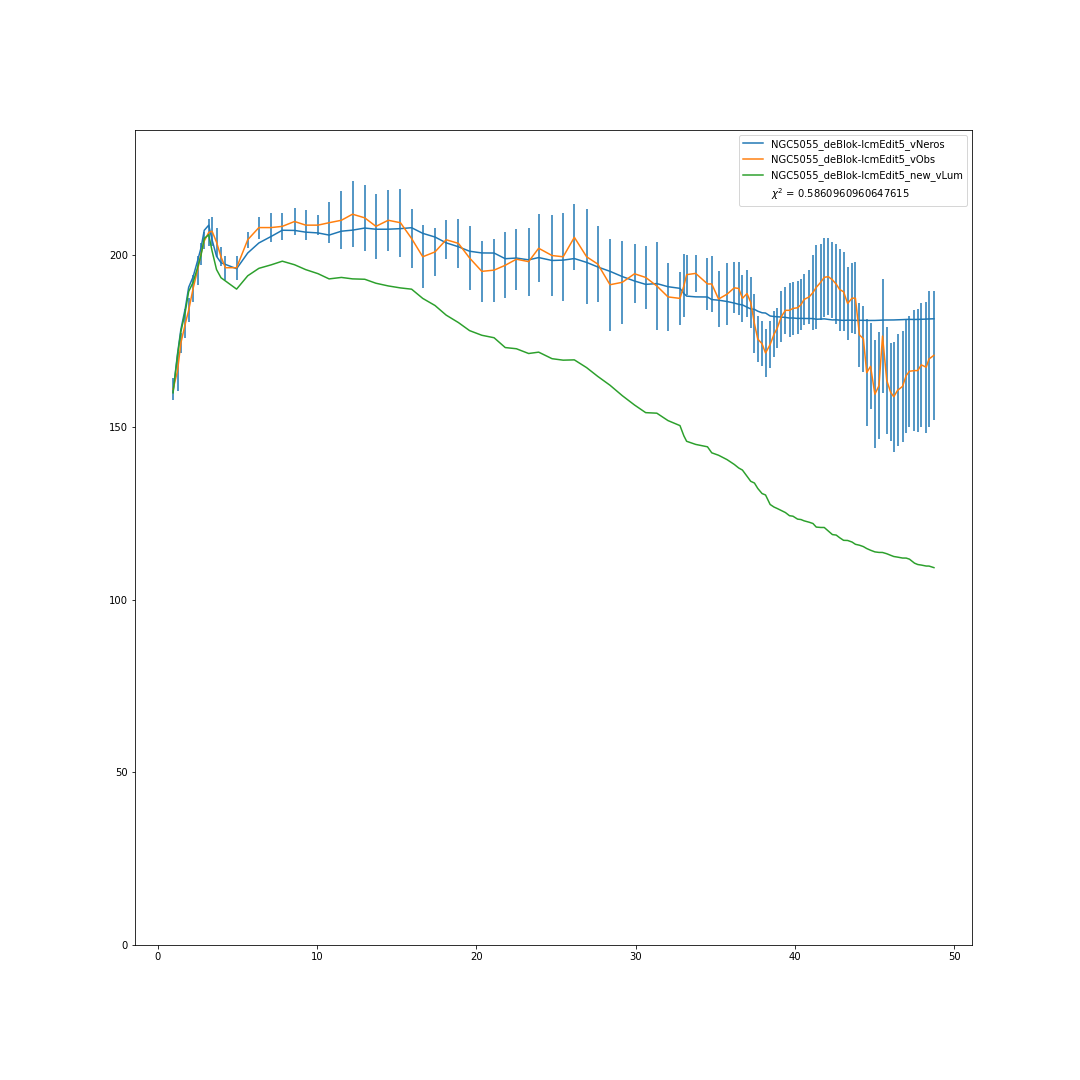
\includegraphics[width=.8\linewidth]{NGC5055_deBlok-lcmEdit5_XueSofue}
  \caption{Lum edits5 \cite{Blok1}}
  \label{fig:sfig3}
\end{subfigure}
\caption{RCFM fits of NGC 5055 }
\label{fig:fig5055}
\end{figure}
 
 
 
  \begin{figure}[h]
\begin{subfigure}{.5\textwidth}
  \centering
  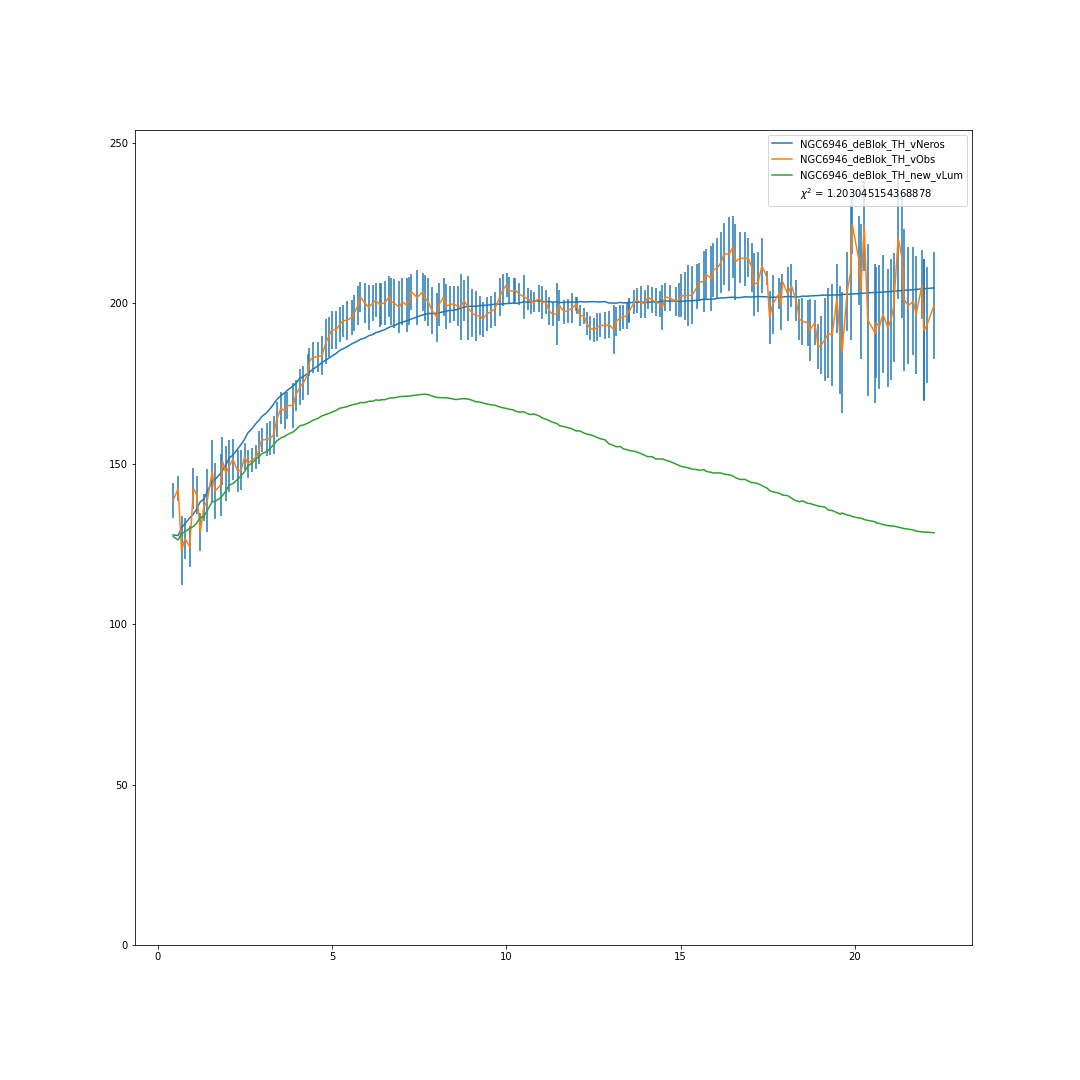
\includegraphics[width=.8\linewidth]{NGC6946_deBlok_TH_XueSofue}
  \caption{deBlok\cite{Blok1}}
  \label{fig:sfig4}
\end{subfigure}%
\begin{subfigure}{.5\textwidth}
  \centering
  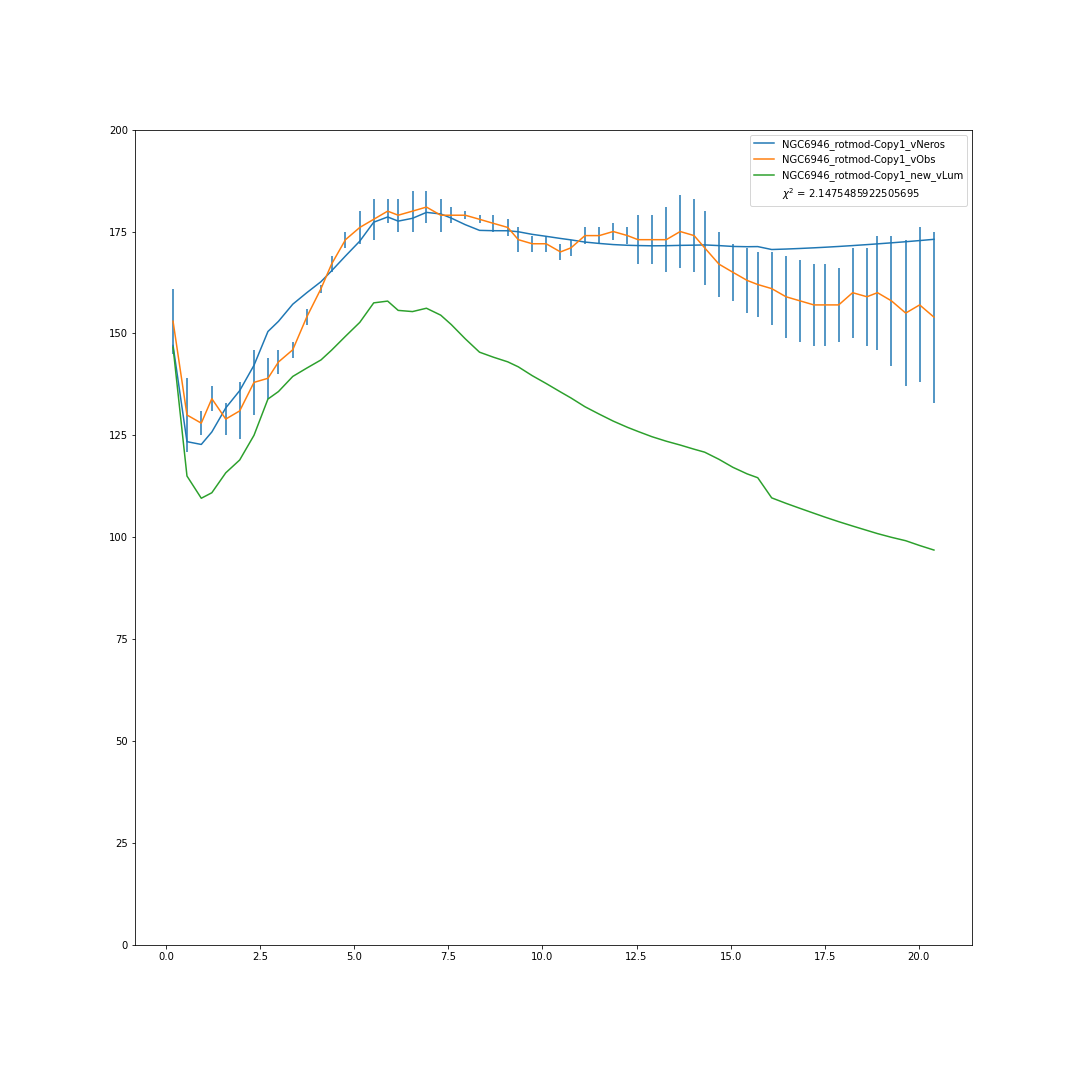
\includegraphics[width=.8\linewidth]{NGC6946_rotmod-Copy1_XueSofue}
  \caption{SPARC\cite{2016Lelli}}
  \label{fig:sfig5}
\end{subfigure}
\caption{RCFM fits  of NGC 6946 }
\label{fig:fig6946}
\end{figure}
%
%
%

  \begin{figure}[h]
\begin{subfigure}{.5\textwidth}
  \centering
  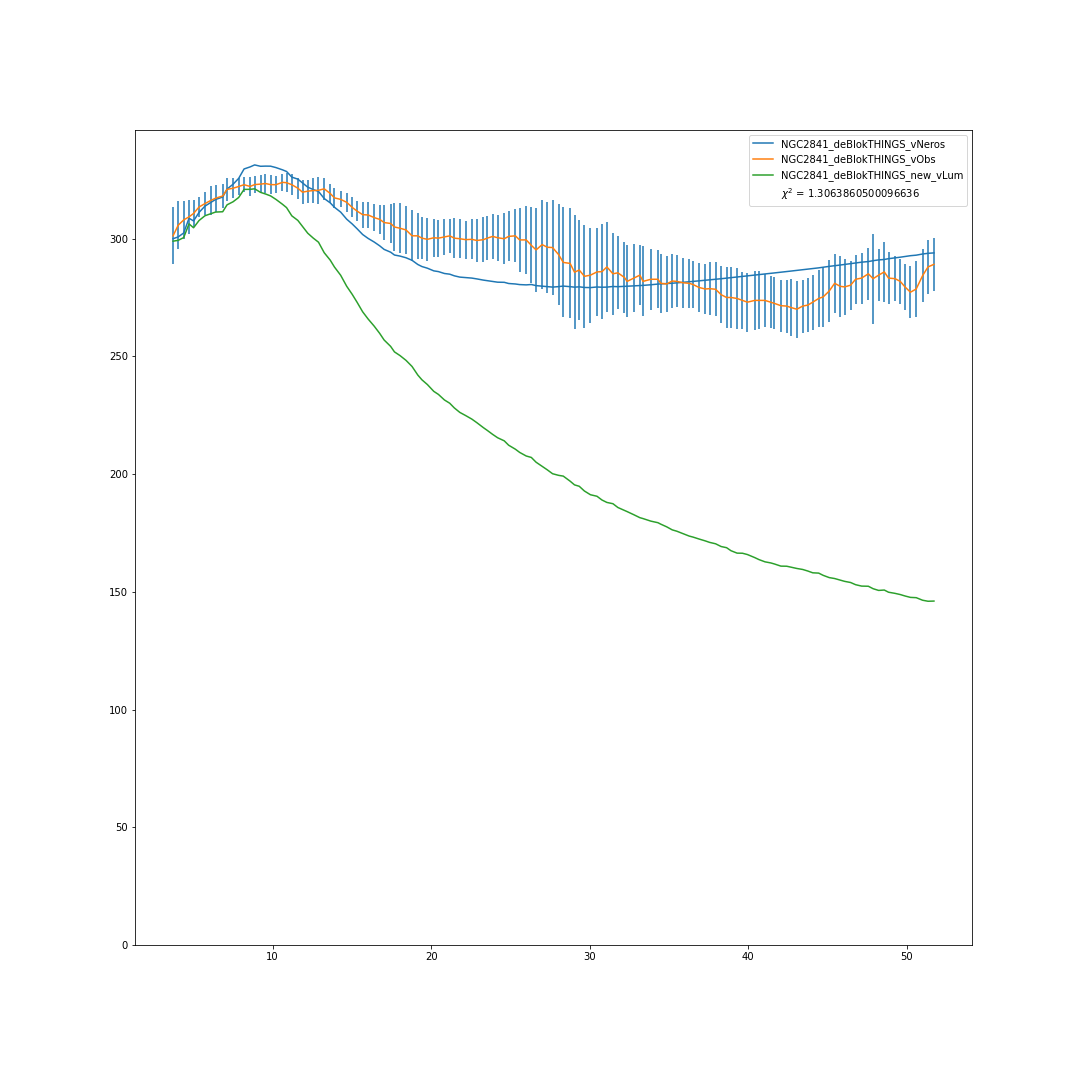
\includegraphics[width=.8\linewidth]{NGC2841_deBlokTHINGS_XueSofue}
  \caption{deBlok\cite{Blok1}}
  \label{fig:sfig9}
\end{subfigure}%
\begin{subfigure}{.5\textwidth}
  \centering
  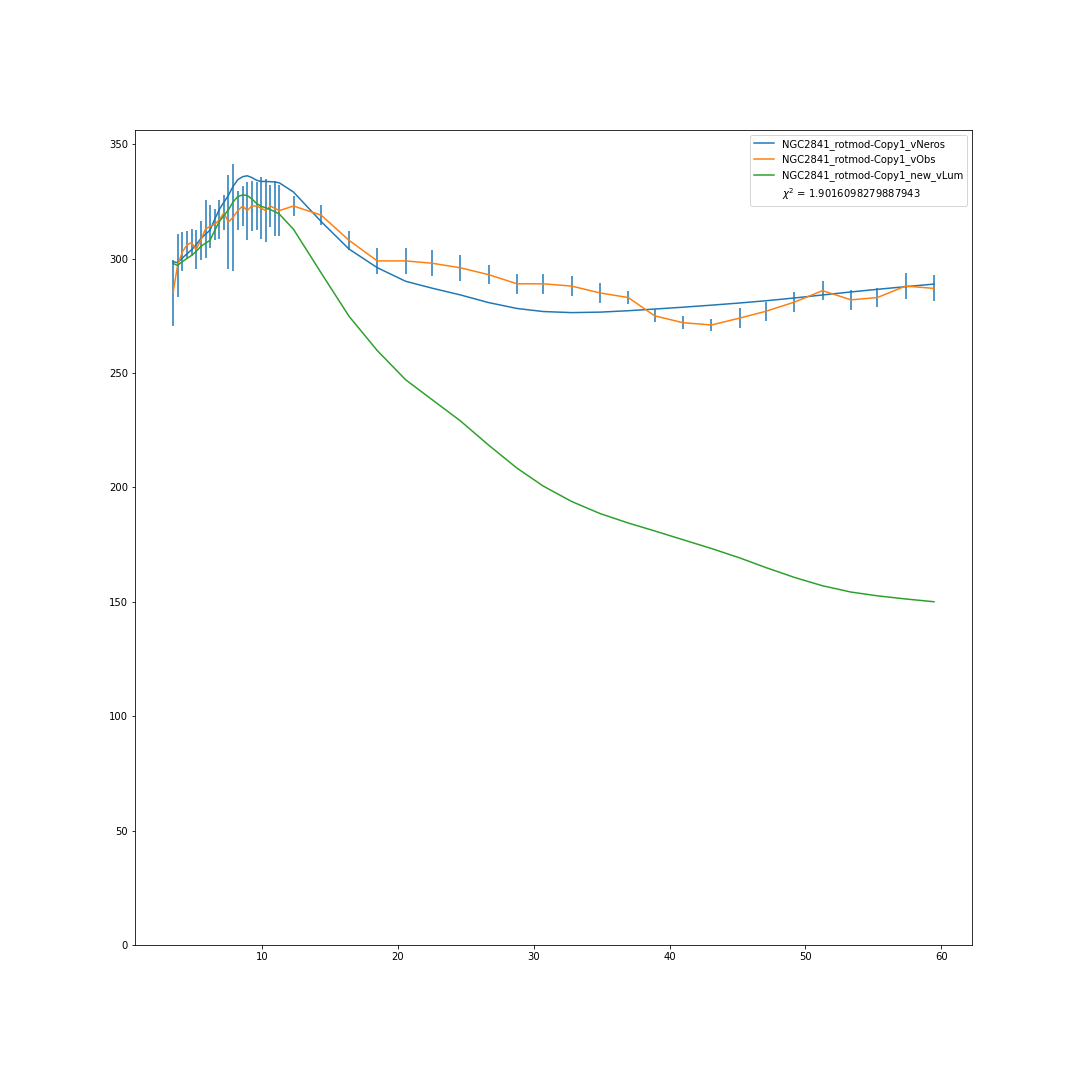
\includegraphics[width=.8\linewidth]{NGC2841_rotmod-Copy1_XueSofue}
  \caption{SPARC\cite{2016Lelli}}
  \label{fig:sfig10}
\end{subfigure}
\caption{RCFM fits  of NGC 2841}
\label{fig:fig2841}
\end{figure}

\clearpage
  \begin{figure}[h]
\begin{subfigure}{.5\textwidth}
  \centering
  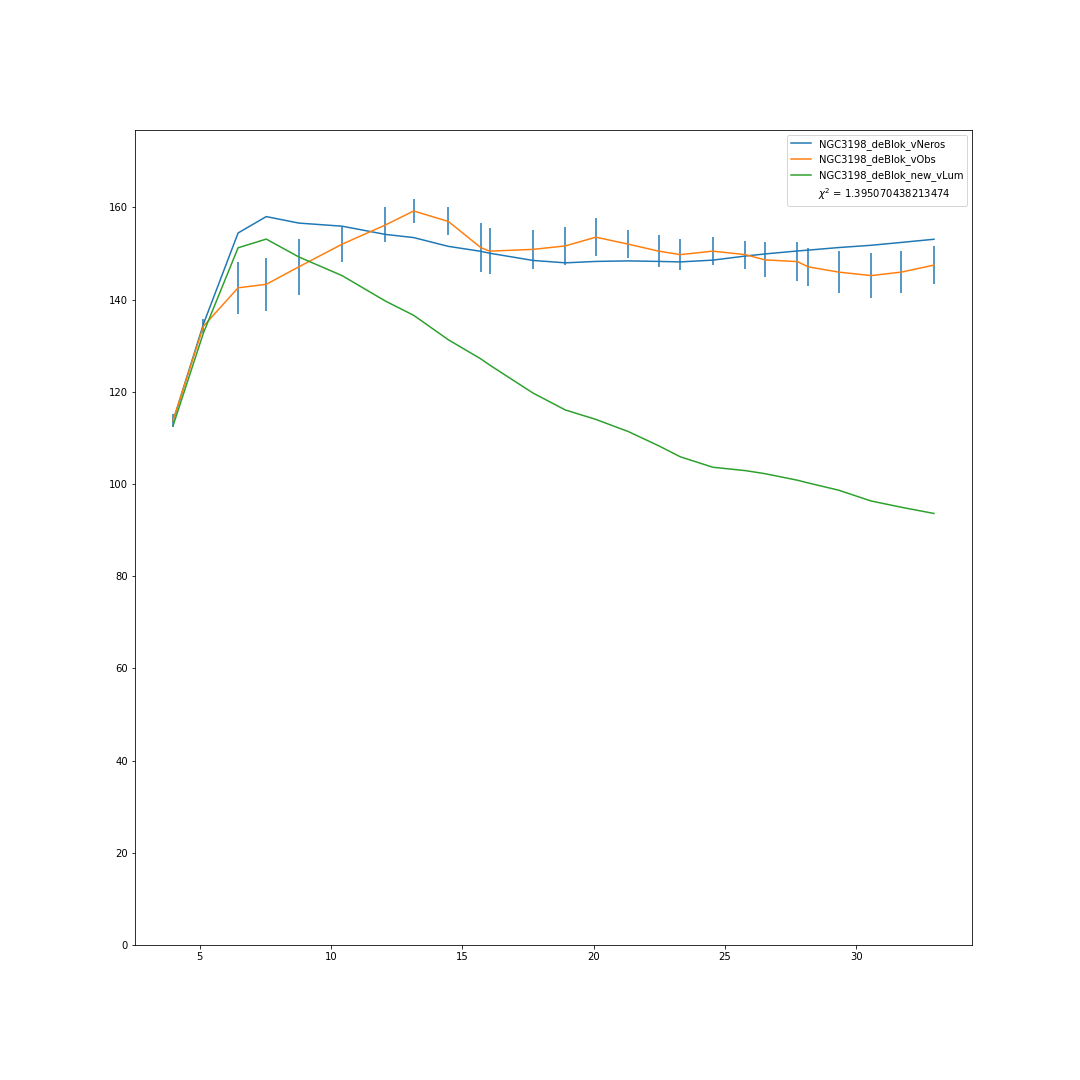
\includegraphics[width=.8\linewidth]{NGC3198_deBlok_XueSofue}
  \caption{deBlok \cite{Blok}}
  \label{fig:sfig6}
\end{subfigure}%
\begin{subfigure}{.5\textwidth}
  \centering
  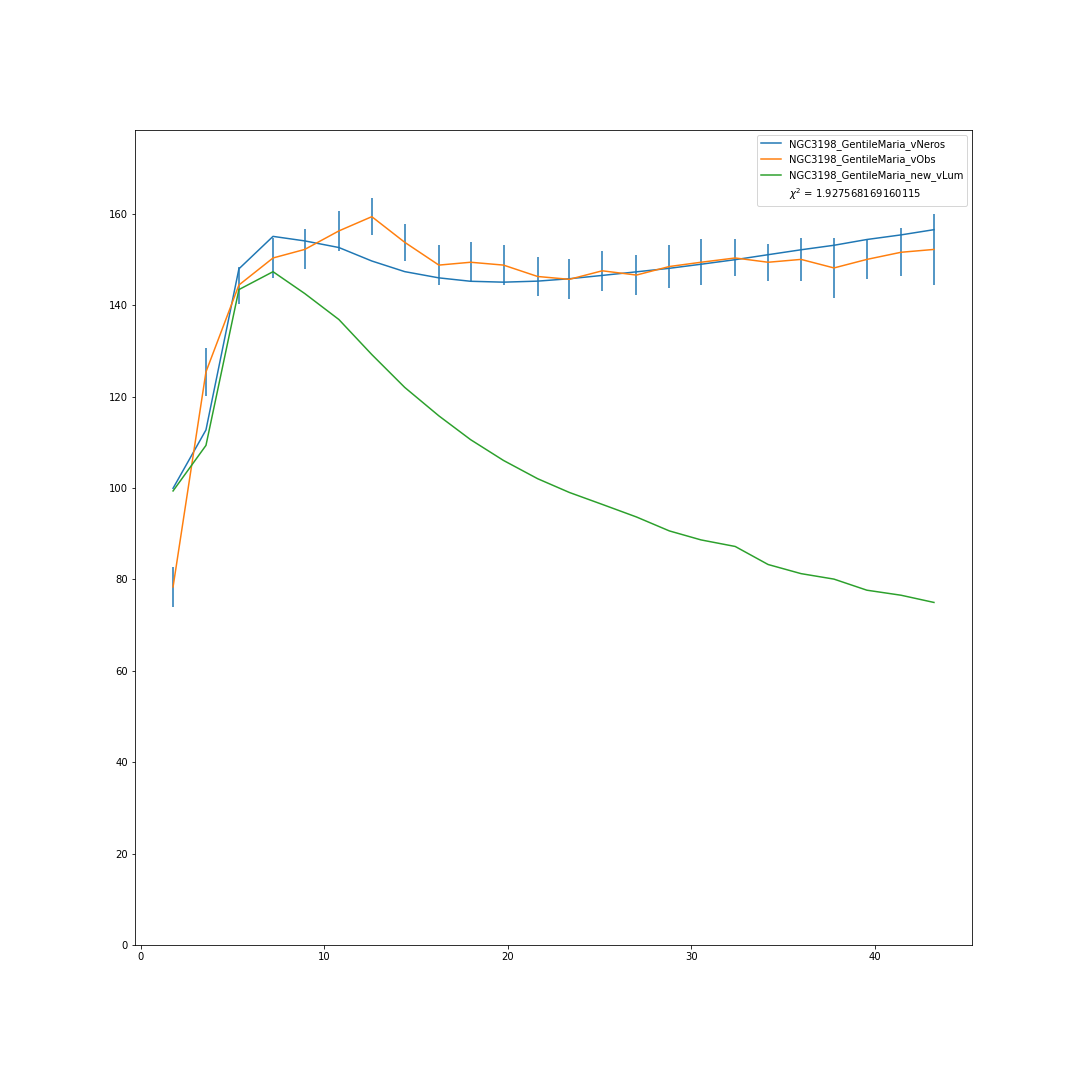
\includegraphics[width=.8\linewidth]{NGC3198_GentileMaria_XueSofue}
  \caption{Gentile \cite{Maria}}
  \label{fig:sfig7}
\end{subfigure}
\begin{subfigure}{.5\textwidth}
  \centering
  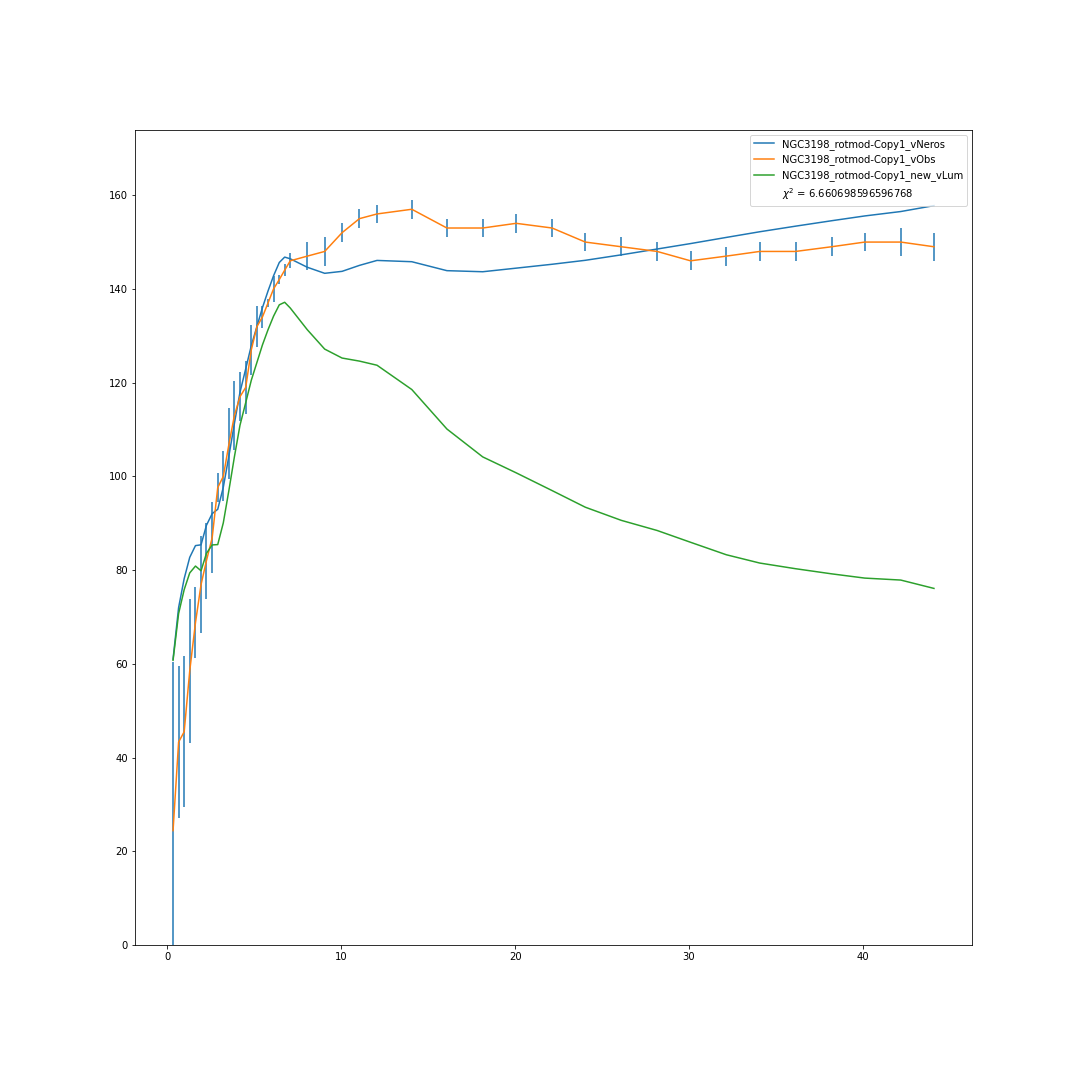
\includegraphics[width=.8\linewidth]{NGC3198_rotmod-Copy1_XueSofue}
  \caption{SPARC\cite{2016Lelli}}
  \label{fig:sfig8}
\end{subfigure}
\caption{RCFM fits  of NGC 3198}
\label{fig:fig3198}
\end{figure}
 %   
%
% 
\clearpage
%%%

  \begin{figure}[h]
\begin{subfigure}{.5\textwidth}
  \centering
  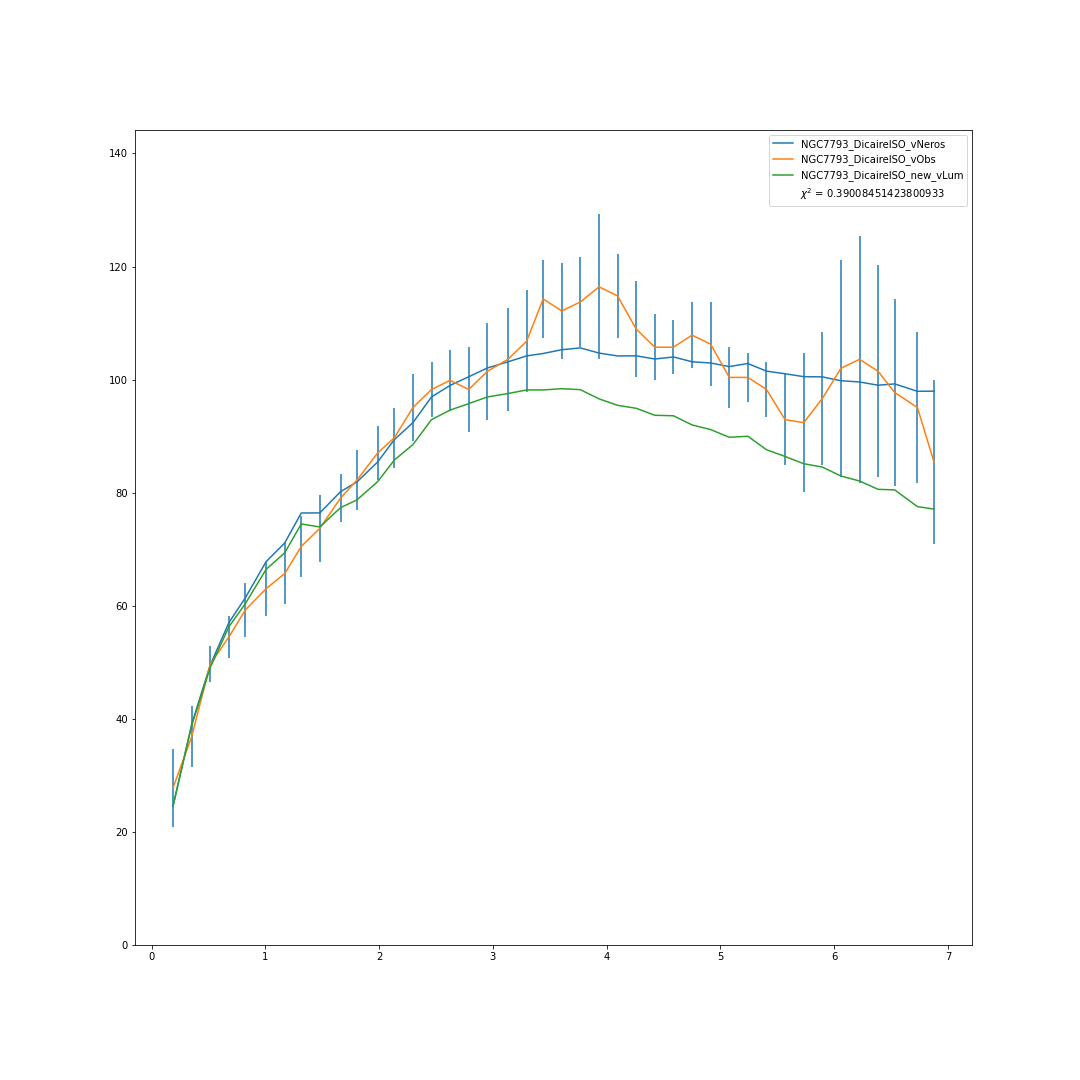
\includegraphics[width=.8\linewidth]{NGC7793_DicaireISO_XueSofue}
  \caption{Dicaire \cite{Dicaire1}}
  \label{fig:sfig11}
\end{subfigure}%
\begin{subfigure}{.5\textwidth}
  \centering
  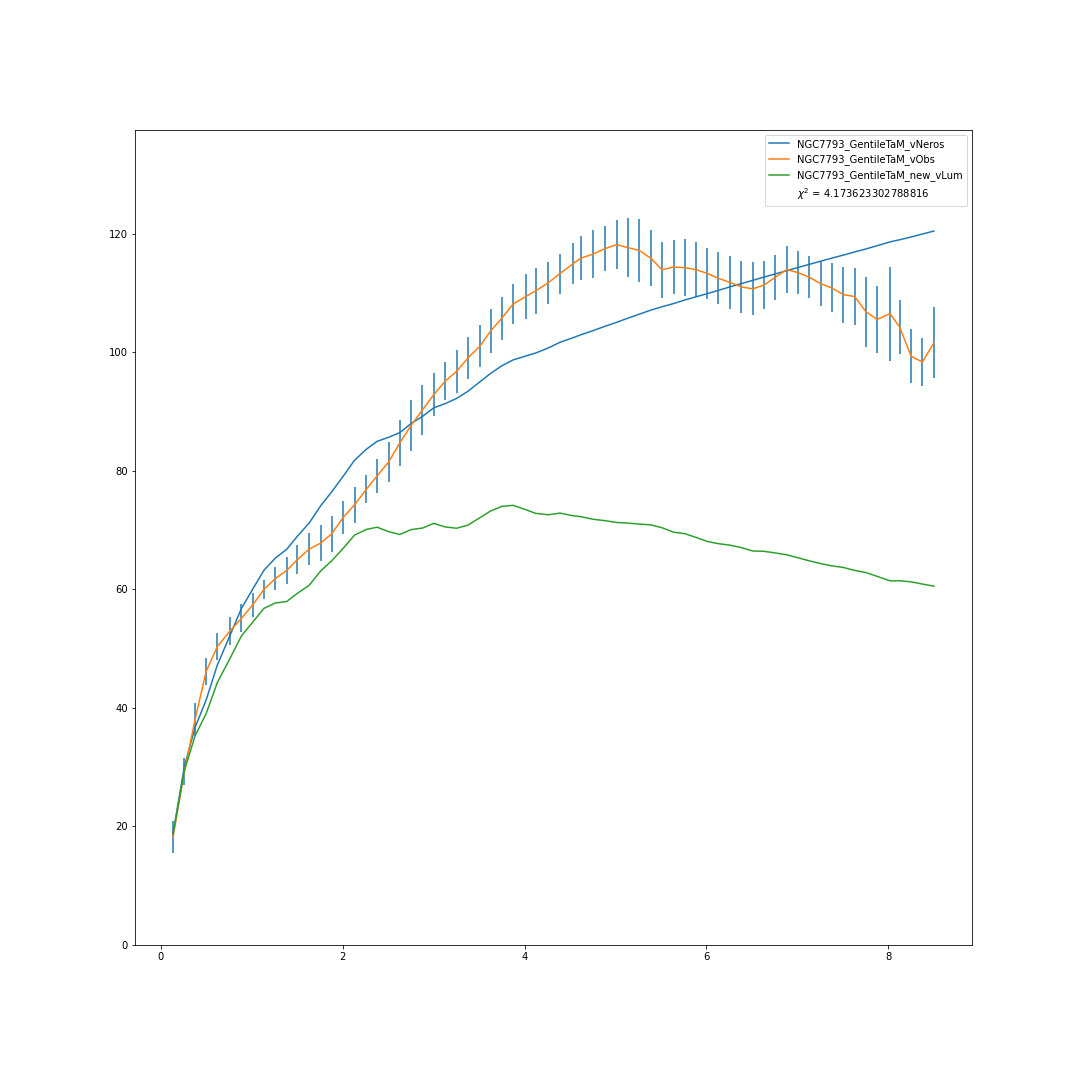
\includegraphics[width=.8\linewidth]{NGC7793_GentileTaM_XueSofue}
  \caption{Gentile\cite{Gent}}
  \label{fig:sfig12}
\end{subfigure}
\begin{subfigure}{.5\textwidth}
  \centering
  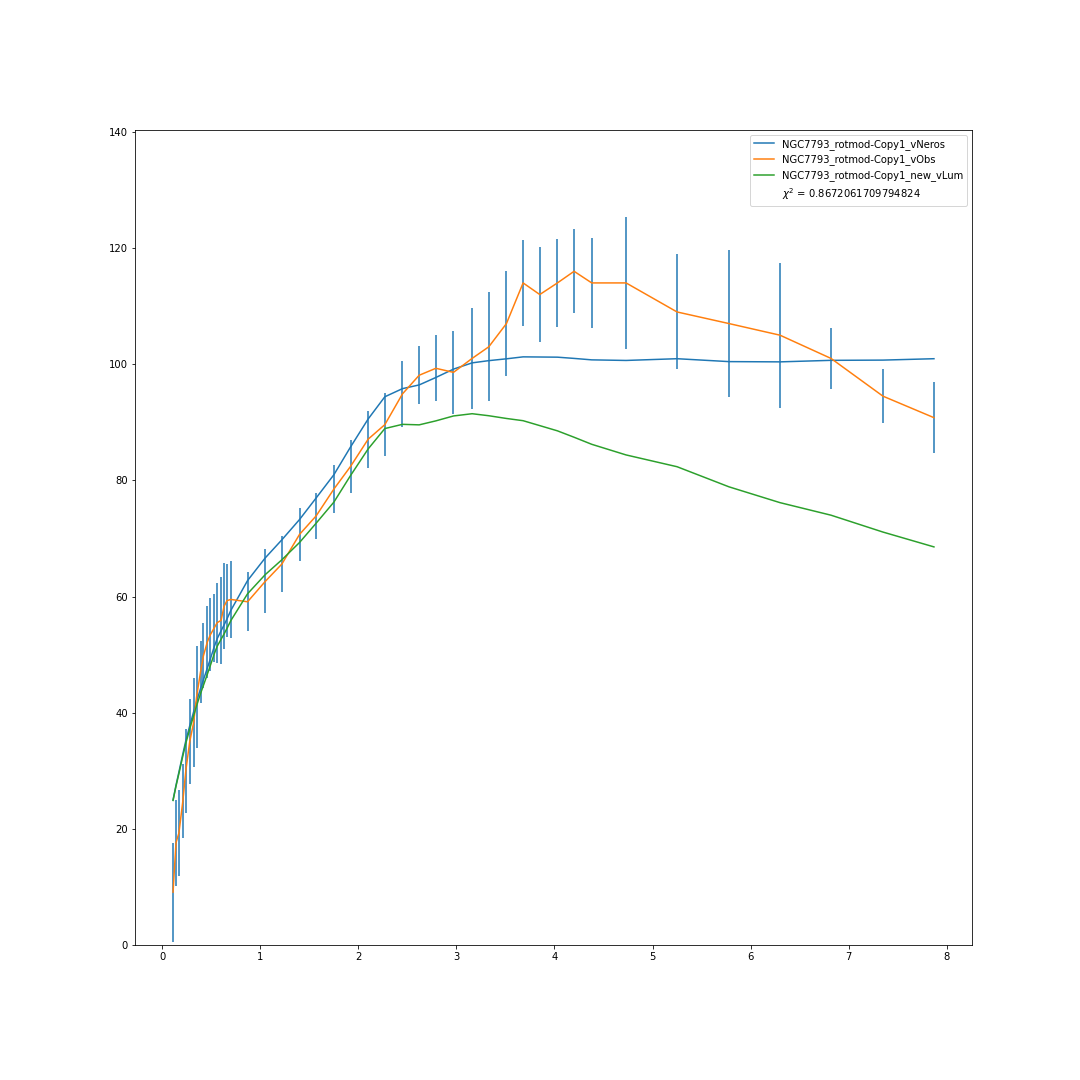
\includegraphics[width=.8\linewidth]{NGC7793_rotmod-Copy1_XueSofue}
  \caption{SPARC\cite{2016Lelli}}
  \label{fig:sfig13}
\end{subfigure}
\caption{RCFM fits  of NGC 7793}
\label{fig:fig7793}
\end{figure}
%
%
%
%
\clearpage
  \begin{figure}[h]
\begin{subfigure}{.5\textwidth}
  \centering
  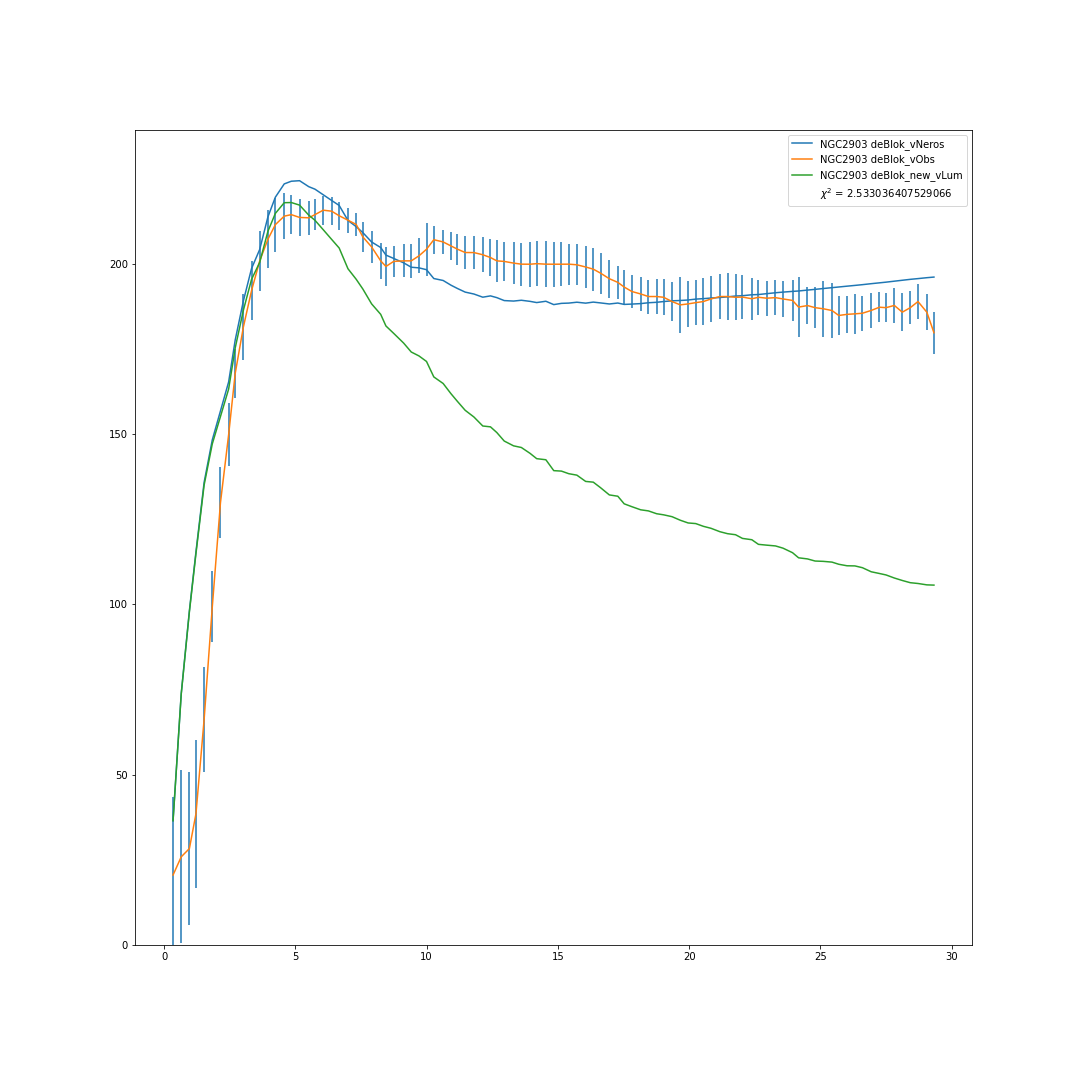
\includegraphics[width=.8\linewidth]{NGC2903deBlok_XueSofue.png}
  \caption{deBlok\cite{Blok1}}
  \label{fig:sfig14}
\end{subfigure}%
\begin{subfigure}{.5\textwidth}
  \centering
  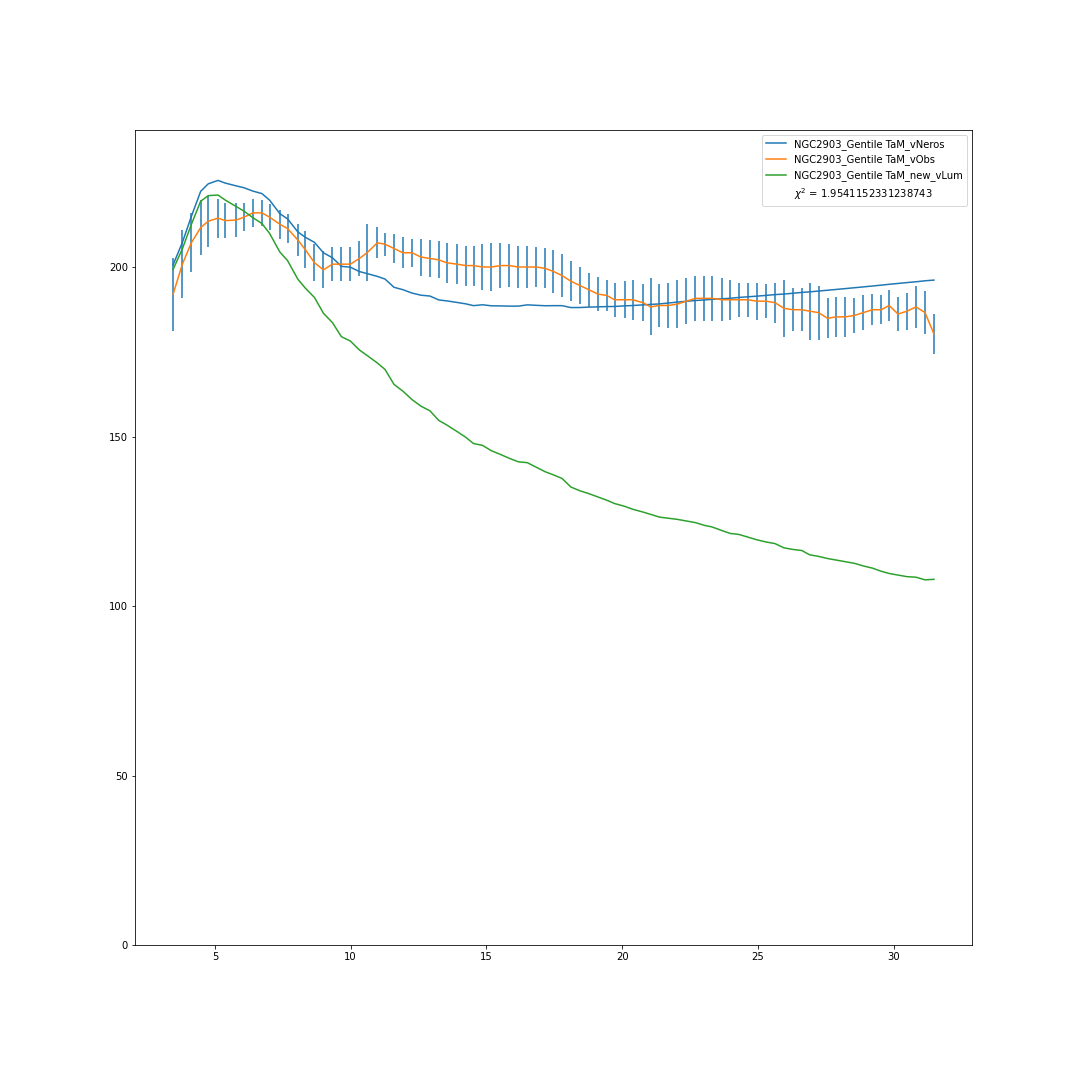
\includegraphics[width=.8\linewidth]{NGC2903_GentileTaM_XueSofue.png}
  \caption{Gentile\cite{Gent}}
  \label{fig:sfig15}
\end{subfigure}
\begin{subfigure}{.5\textwidth}
  \centering
  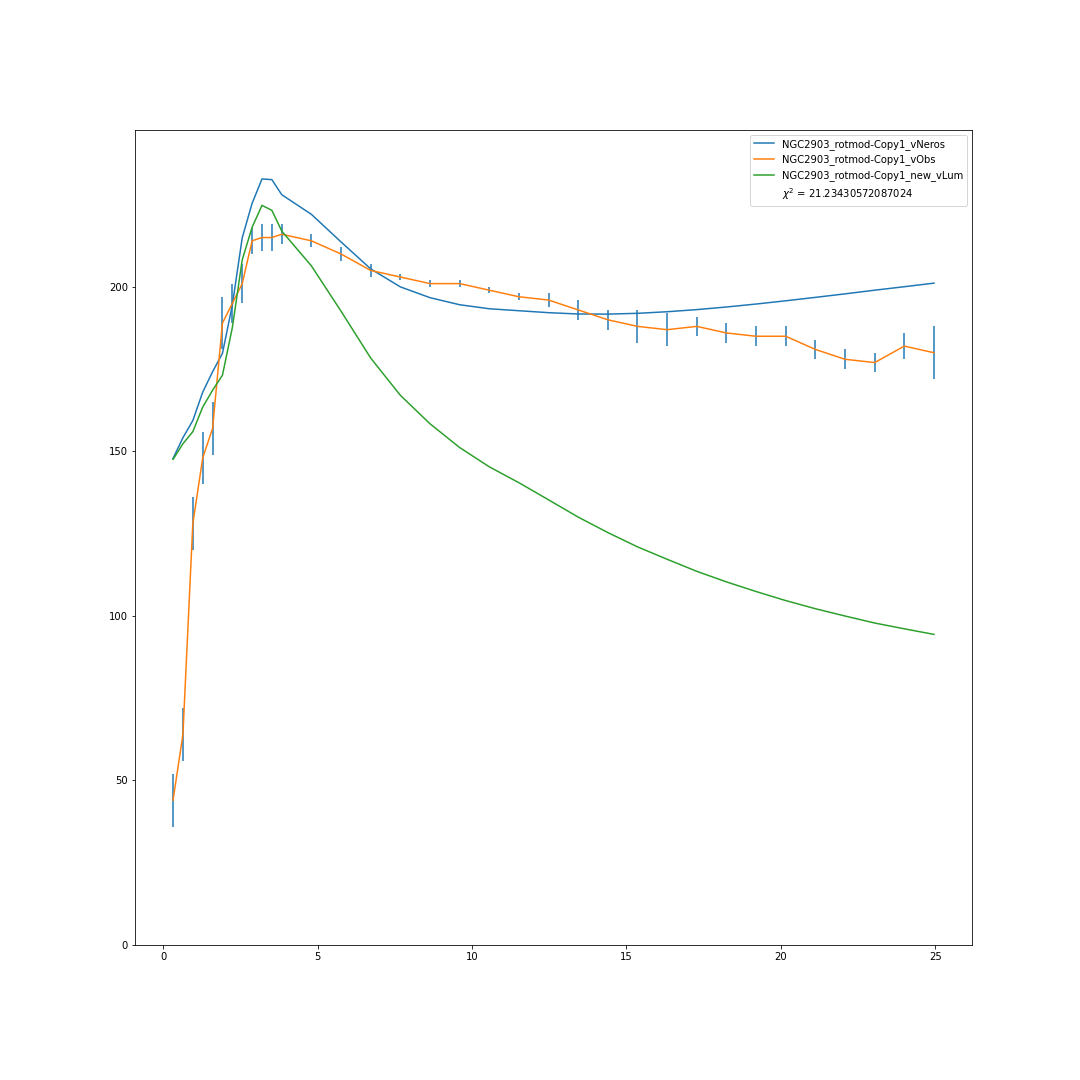
\includegraphics[width=.8\linewidth]{NGC2903_rotmod-Copy1_XueSofue.png}
  \caption{SPARC\cite{2016Lelli}}
  \label{fig:sfig16}
\end{subfigure}
\caption{plots of NGC 2903}
\label{fig:fig2903}
\end{figure}
%
\clearpage
%
%  
  \begin{figure}[h]
\begin{subfigure}{.5\textwidth}
  \centering
  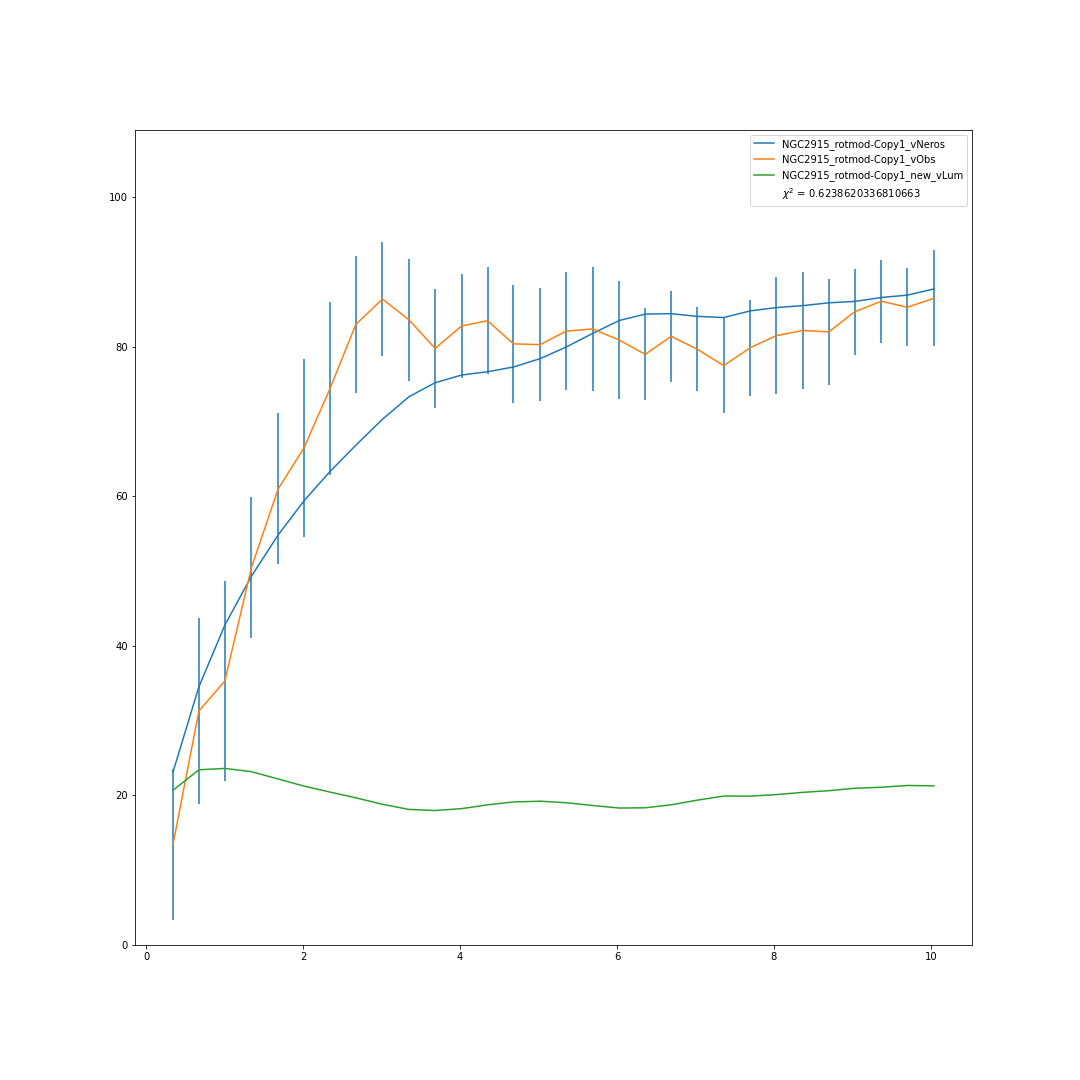
\includegraphics[width=.8\linewidth]{NGC2915_rotmod-Copy1_XueSofue.png}
  \caption{SPARC\cite{2016Lelli}}
  \label{fig:sfig17}
\end{subfigure}%
\begin{subfigure}{.5\textwidth}
  \centering
  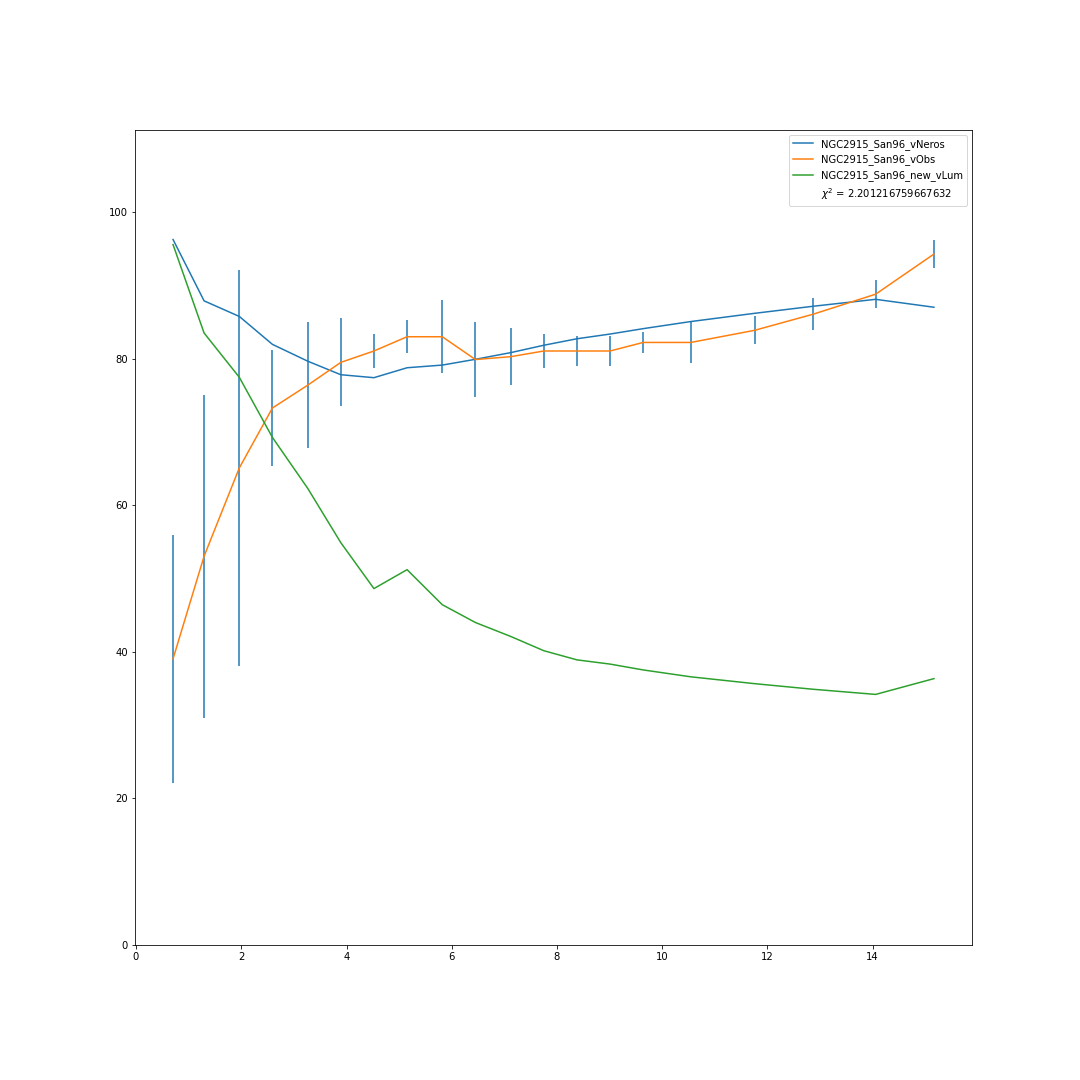
\includegraphics[width=.8\linewidth]{NGC2915_San96_XueSofue.png}
  \caption{Sanders\cite{San96}}
  \label{fig:sfig18}
\end{subfigure}
\caption{plots of NGC 2915}
\label{fig:fig2915}
\end{figure}
%
%
%
%  
%%%%%%%
  \begin{figure}[h]
\begin{subfigure}{.5\textwidth}
  \centering
  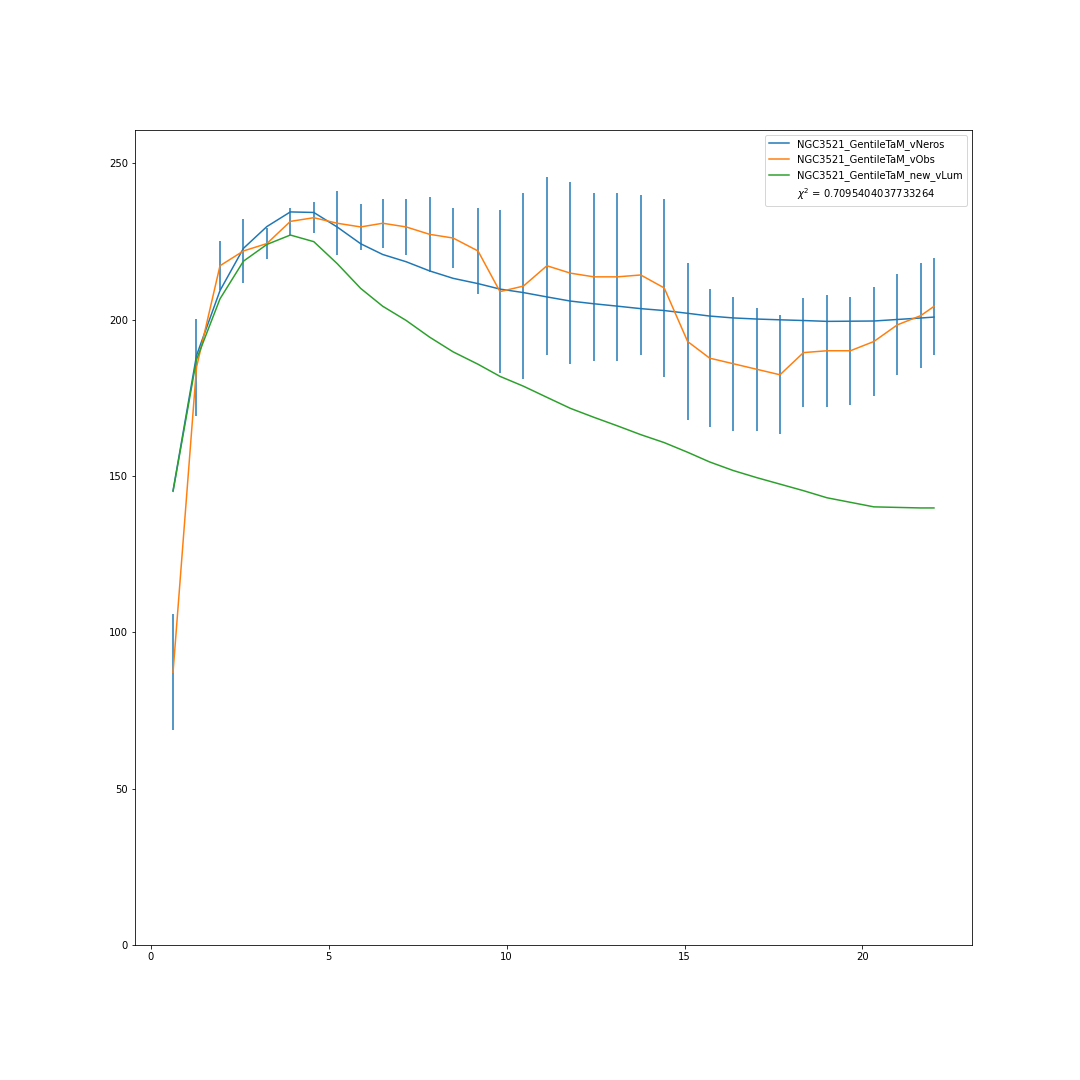
\includegraphics[width=.8\linewidth]{NGC3521_GentileTaM_XueSofue.png}
  \caption{Gentile\cite{Gent}}
  \label{fig:sfig19}
\end{subfigure}%
\begin{subfigure}{.5\textwidth}
  \centering
  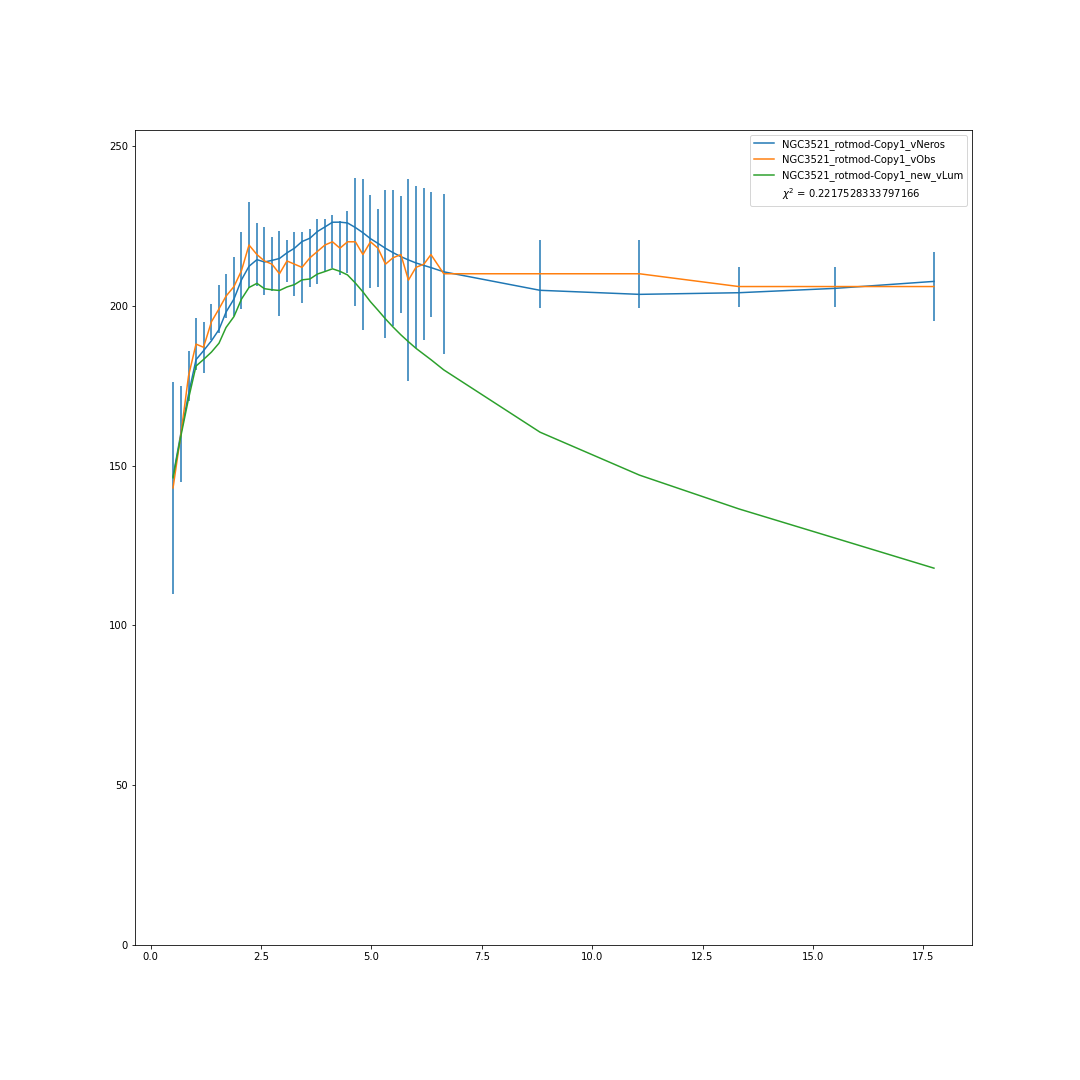
\includegraphics[width=.8\linewidth]{NGC3521_rotmod-Copy1_XueSofue.png}
  \caption{SPARC\cite{2016Lelli}}
  \label{fig:sfig20}
\end{subfigure}
\caption{plots of NGC 3521}
\label{fig:fig3521}
\end{figure}
%
%
%
\clearpage
 \begin{figure}[h]
\begin{subfigure}{.5\textwidth}
  \centering
  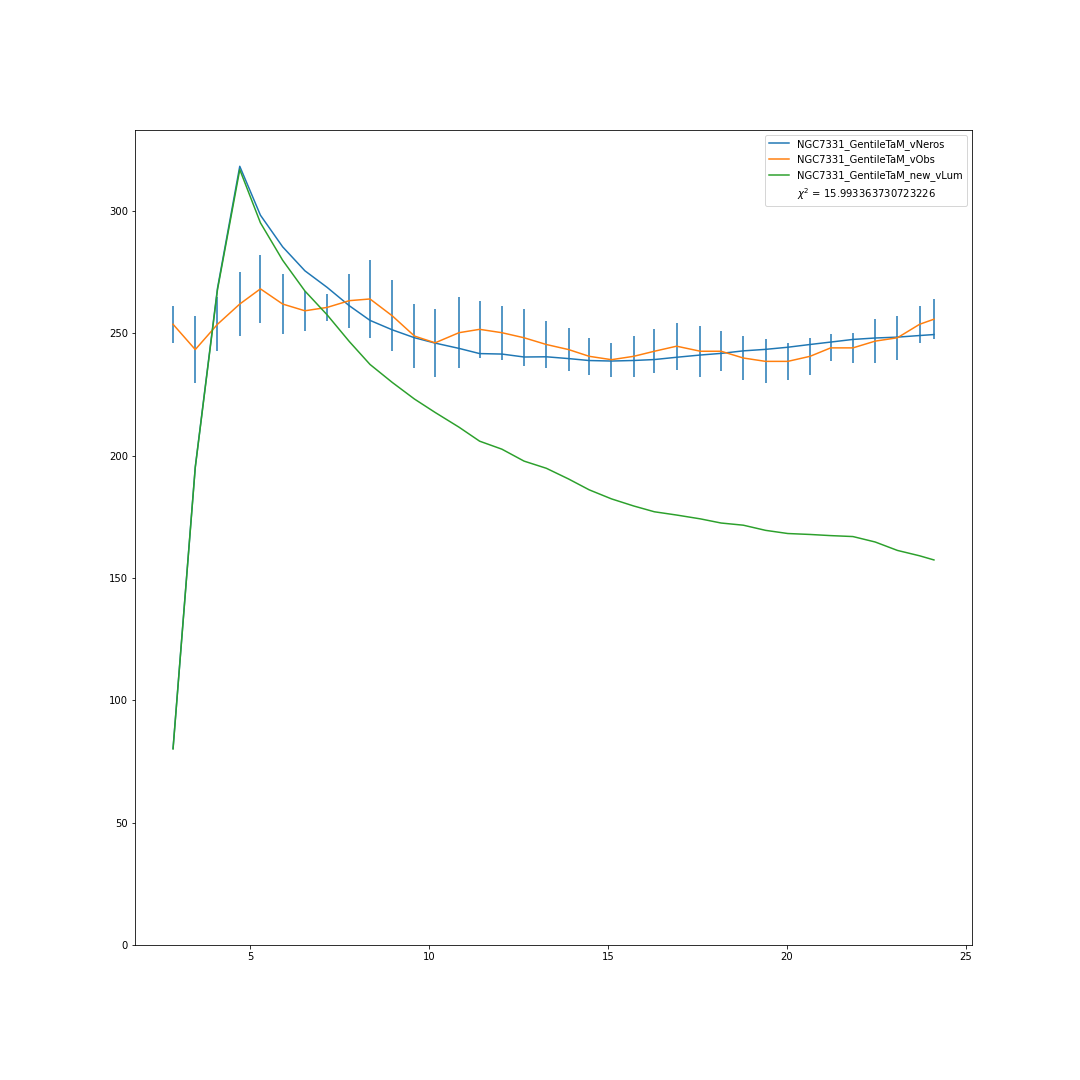
\includegraphics[width=.8\linewidth]{NGC7331_GentileTaM_XueSofue.png}
  \caption{Gentile\cite{Gent}}
  \label{fig:sfig21}
\end{subfigure}%
\begin{subfigure}{.5\textwidth}
  \centering
  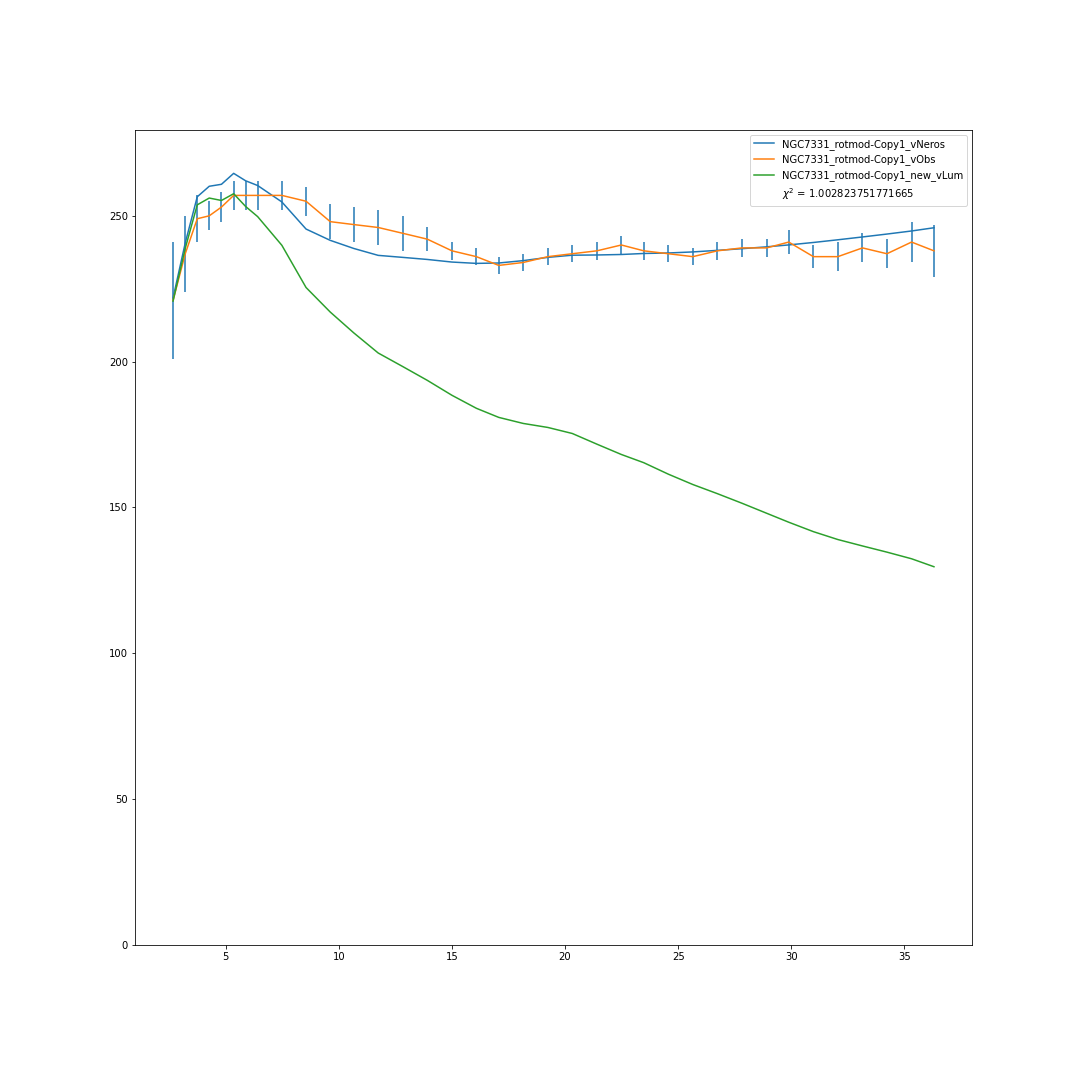
\includegraphics[width=.8\linewidth]{NGC7331_rotmod-Copy1_XueSofue.png}
  \caption{SPARC\cite{2016Lelli}}
  \label{fig:sfig22}
\end{subfigure}
\caption{plots of NGC 7331}
\label{fig:fig7331}
\end{figure}
%%%%%%%
 \begin{figure}[h]
\begin{subfigure}{.5\textwidth}
  \centering
  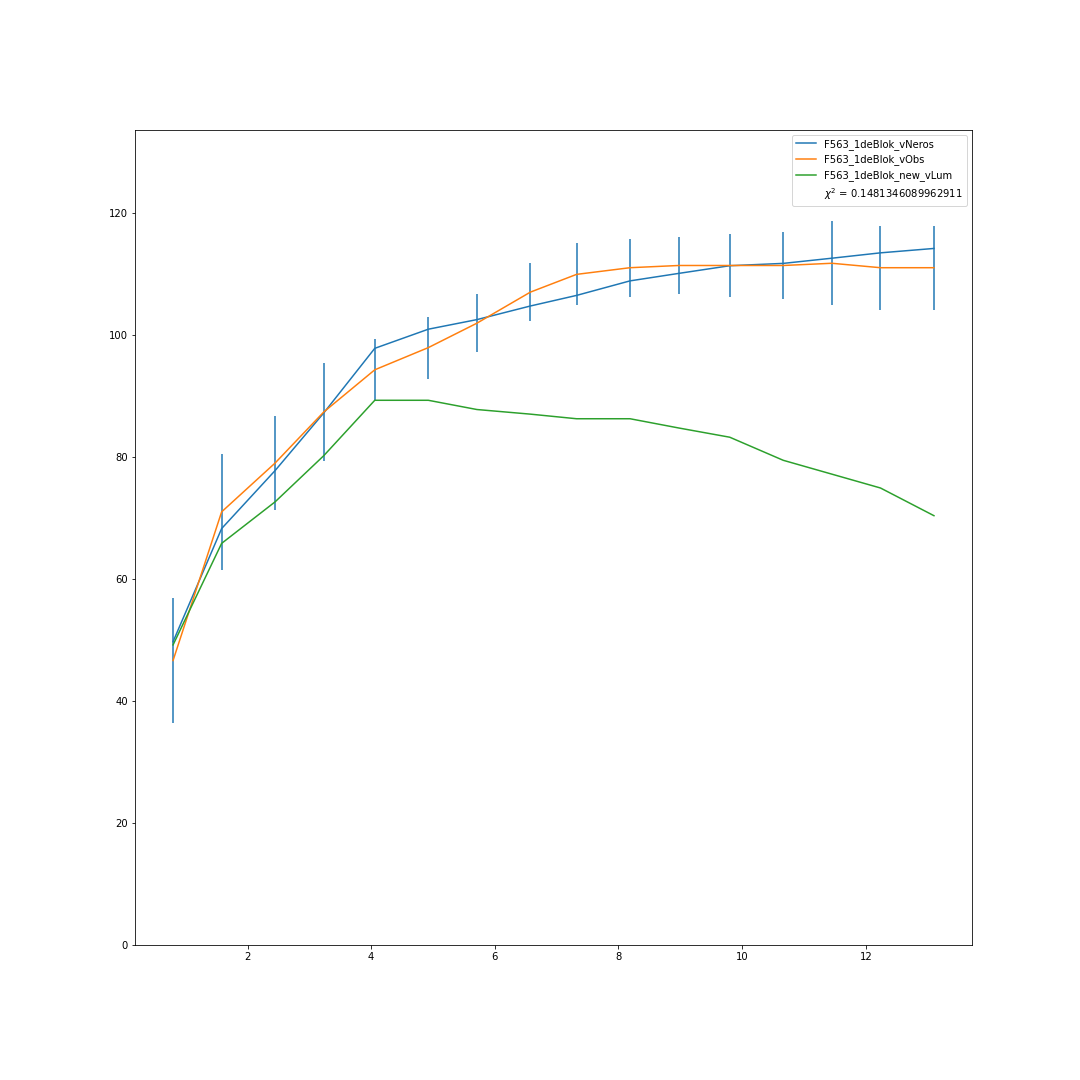
\includegraphics[width=.8\linewidth]{F563_1deBlok_XueSofue.png}
  \caption{de Blok}
  \label{fig:sfig23}
\end{subfigure}%
\begin{subfigure}{.5\textwidth}
  \centering
  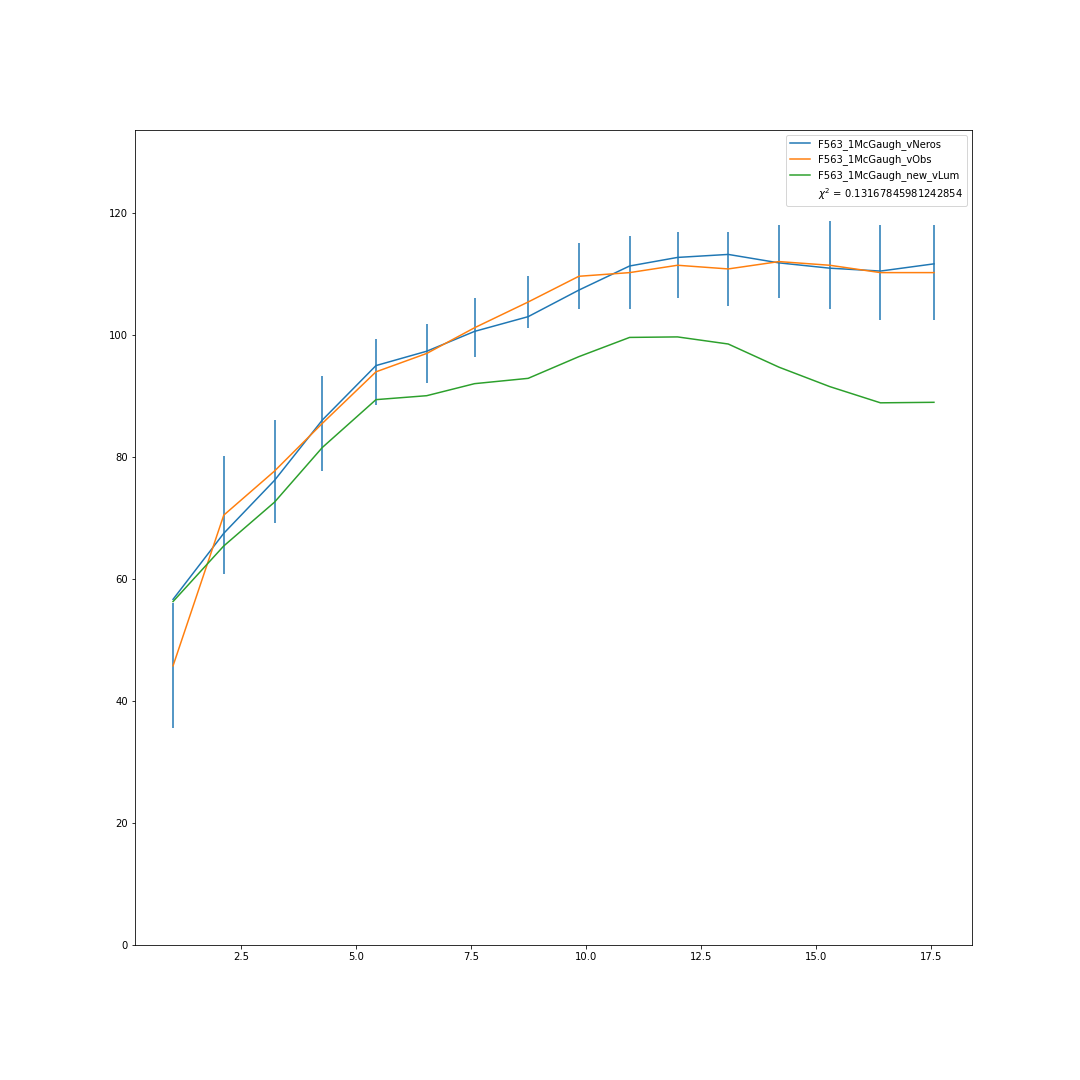
\includegraphics[width=.8\linewidth]{F563_1McGaugh_XueSofue.png}
  \caption{McGaugh}
  \label{fig:sfig24}
\end{subfigure}
\caption{plots of F563-1}
\label{fig:figF563-1}
\end{figure}
\clearpage
%%%%%%
%%%%%%%%
%%%%%%
%%%%%%%
%%%%%%
  
 
\begin{figure*}
    \centering
    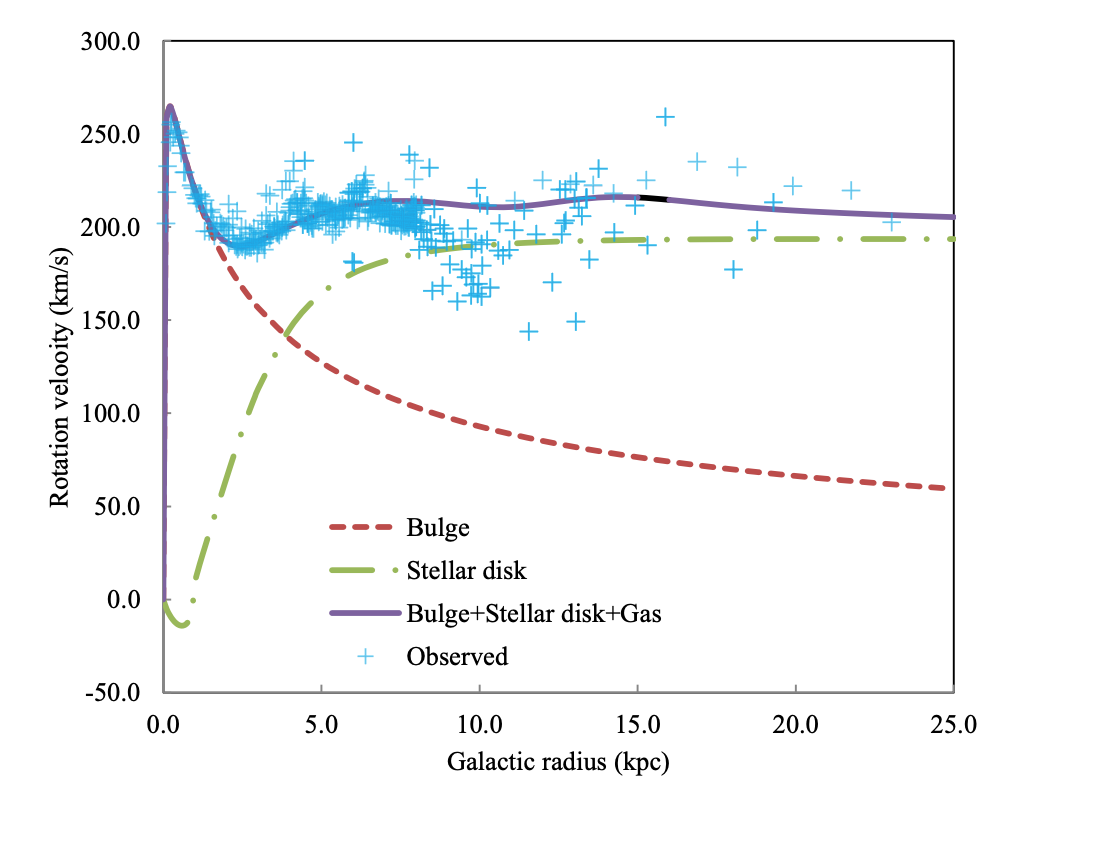
\includegraphics{MW_Enbang_Li}
    \caption{Enbang Li \cite{Li2016ModellingMD}}
    \label{fig:my_label}
\end{figure*}

    
     

\bibliography{LCM} 

\end{document}
%
% ****** End of file apssamp.tex ******